	%сделать восклицательный знак
\documentclass[a4paper,12pt,fleqn]{article} % добавить leqno в [] для нумерации слева

%%% Работа с русским языком
\usepackage{cmap}					% поиск в PDF
\usepackage{mathtext} 				% русские буквы в формулах
\usepackage[T2A]{fontenc}			% кодировка
\usepackage[utf8]{inputenc}			% кодировка исходного текста
\usepackage[english,russian]{babel}	% локализация и переносы

%%% Дополнительная работа с математикой
\usepackage{amsmath,amsfonts,amssymb,amsthm,mathtools} % AMS
\usepackage{icomma} % "Умная" запятая

%% Номера формул
%\mathtoolsset{showonlyrefs=true} % Показывать номера только у тех формул, на которые есть \eqref{} в тексте.
%\usepackage{leqno} %Нумерация формул слева

%% Шрифты
\usepackage{euscript}	 % Шрифт Евклид
\usepackage{mathrsfs} % Красивый матшрифт


%% Свои команды
\DeclareMathOperator{\sgn}{\mathop{sgn}}

%% Перенос знаков в формулах (по Львовскому)
\newcommand*{\hm}[1]{#1\nobreak\discretionary{}
{\hbox{$\mathsurround=0pt #1$}}{}}

%%% Заголовок
\author{}
\title{}
\date{}



%%% Теоремы
%\theoremstyle{definition}
%\newtheorem{case}{Задача}[section]
%\renewcommand{\thecase}{\arabic{case}}

%\theoremstyle{definition} % "Определение"
%\newtheorem{corollary}{Пункт}[case]
%\newtheorem{problem}{Задача}[section]
%\renewcommand{\thecorollary}{\asbuk{corollary}}

\usepackage{multicol} % Несколько колонок


%%% Работа с картинками
\usepackage{graphicx}  % Для вставки рисунков
\graphicspath{{images/}{images2/}}  % папки с картинками
\setlength\fboxsep{3pt} % Отступ рамки \fbox{} от рисунка
\setlength\fboxrule{1pt} % Толщина линий рамки \fbox{}
\usepackage{wrapfig} % Обтекание рисунков текстом

%%% Работа с таблицами
\usepackage{array,tabularx,tabulary,booktabs} % Дополнительная работа с таблицами
\usepackage{longtable}  % Длинные таблицы
\usepackage{multirow} % Слияние строк в таблице

%%% Страница
%\usepackage{extsizes} % Возможность сделать 14-й шрифт
\usepackage{geometry} % Простой способ задавать поля
\geometry{top=20mm}
\geometry{bottom=20mm}
\geometry{left=30mm}
\geometry{right=20mm}
%
\usepackage{fancyhdr} % Колонтитулы
\pagestyle{fancy}
\renewcommand{\headrulewidth}{0.1mm}  % Толщина линейки, отчеркивающей верхний колонтитул
%\lfoot{Нижний левый}
%\rfoot{Нижний правый}
\rhead{Глава \thesection}
%\chead{Верхний в центре}
%\lhead{}
% \cfoot{Нижний в центре} % По умолчанию здесь номер страницы

\usepackage{setspace} % Интерлиньяж
%\onehalfspacing % Интерлиньяж 1.5
%\doublespacing % Интерлиньяж 2
%\singlespacing % Интерлиньяж 1

\usepackage{soulutf8} % Модификаторы начертания
\usepackage{bm} % Модификатор начертания для математики

%\usepackage{tikz} % Работа с графикой
%\usepackage{pgfplots}
%\usepackage{pgfplotstable}
%\usepackage[utf8]{inputenc}
%\usetikzlibrary{arrows}


\usepackage{hyperref}
\usepackage[usenames,dvipsnames,svgnames,table,rgb]{xcolor}
\hypersetup{				% Гиперссылки
	unicode=true,           % русские буквы в раздела PDF
	pdftitle={Заголовок},   % Заголовок
	pdfauthor={Автор},      % Автор
	pdfsubject={Тема},      % Тема
	pdfcreator={Создатель}, % Создатель
	pdfproducer={Производитель}, % Производитель
	pdfkeywords={keyword1} {key2} {key3}, % Ключевые слова
	colorlinks=true,       	% false: ссылки в рамках; true: цветные ссылки
	linkcolor=blue!55!red,          % внутренние ссылки
	citecolor=green,        % на библиографию
	filecolor=magenta,      % на файлы
	urlcolor=blue          % на URL
} 
\usepackage{datetime}
\newdateformat{onlyyear}{\THEYEAR}
\newdateformat{defaultdate}{\THEDAY~\monthname[\THEMONTH] \THEYEAR~г.}

\usepackage{multicol} % Несколько колонок

\usepackage{indentfirst} % Красная строка

\usepackage{tikz} % Работа с графикой
\usepackage{pgfplots} %взять данные из соседнего файла и построить по ним что-либо
\usepackage{pgfplotstable}
\usetikzlibrary{fadings}
\usetikzlibrary{decorations}
\usepgflibrary{decorations.pathmorphing}

\tikzfading[name=fade out, inner color=transparent!0,
outer color=transparent!100]

\usepackage[utf8]{inputenc}
\usetikzlibrary{arrows}
\usepackage{tcolorbox}
\usepackage{lipsum}
\tcbuselibrary{breakable}

%\usetikzlibrary{calc}

\usepackage{xparse}
\NewDocumentCommand{\definition}{mm}{ \textbf{Определение.} \textit{#1} --- #2 \vspace{0.3cm}}

\renewcommand{\familydefault}{\sfdefault}
\usepackage{float}

\usepackage{relsize}
\newcommand{\bigem}[1][1]{\text{\larger[#1]{\color{blue!55!red}{ \textbf{$ ! $}}}}}


\begin{document} % конец преамбулы, начало документа
	
\tableofcontents

\newpage


\section{Угрозы в области физической безопасности}

\begin{tcolorbox}[colback=blue!40!red!10!,colframe=blue!40!red]

В результате изучения главы студент должен \textbf{знать} основные угрозы в области обеспечения физической безопасности предприятия в сферах защиты жизни и здоровья физических лиц, обеспечения сохранности финансовых и иных материальных ценностей, а также объектов недвижимости; \textbf{уметь} сопоставлять основные угрозы с типовыми мерами обеспечения физической защиты бизнеса; \textbf{владеть} методами обеспечения физической безопасности предприятия с применением различных типов защиты, а также расчетом экономических показателей себестоимости различных вариантов охраны.

\end{tcolorbox}


\subsection{Угроза жизни и здоровью физических лиц}

Важным \textit{условием успешного функционирования любого предприятия на рынке} является защита от возникающих угроз, среди которых особую опасность представляют незаконные действия физических лиц. Последствия их действий непредсказуемы: от хищения имущества до создания чрезвычайных ситуаций на объекте. В этих условиях безопасность любого субъекта рынка осуществляется на основе принципов «разумной достаточности», «эффективность – стоимость», а также разработанной в теории и применяемой на практике концепции физической безопасности предприятия.

В рамках единой политики безопасности организации физическая безопасность является основным структурным элементом, направленным на сохранение собственности, жизни и здоровья персонала, финансовых ресурсов.\\

\definition{Физическая безопасность организации} {совокупность правовых норм, организационных мер и инженерно-технических решений, направленных на защиту важных интересов и ресурсов предприятия (объекта) от угроз злоумышленных противоправных действий физических лиц (нарушителей или злоумышленников).}

Как правило, она включает в себя силы подразделений безопасности и охраны объекта, комплекс инженерно-технических средств охраны, а также режим, установленный на объекте. Система физической защиты не должна препятствовать нормальному функционированию организации, ее технологическим процессам.

Угрозы в области физической безопасности существенно различаются по своей тяжести и зависят от возможностей и способностей нарушителя. В качестве \textit{основных видов угроз в области физической безопасности} принято различать  (см. рисунок \ref{image1}): 

\begin{itemize}
	\item Чрезвычайные ситуации (пожар, разрушение, затопление, авария, хищение опасных веществ, массовые инфекционные заболевания и отравления людей и т.п.);
	\item Промышленный шпионаж;
	\item Угрозы физическому лицу (сотрудникам): причинение вреда здоровью, причинение увечий, создание угроз для жизни;
	\item Хищение или порча имущества;
	\item Несанкционированный съем информации, содержащей государственную, служебную или коммерческую тайны;
	\item Снижение эффективности функционирования и устойчивости развития предприятия.
\end{itemize}

\begin{figure}
	\centering
	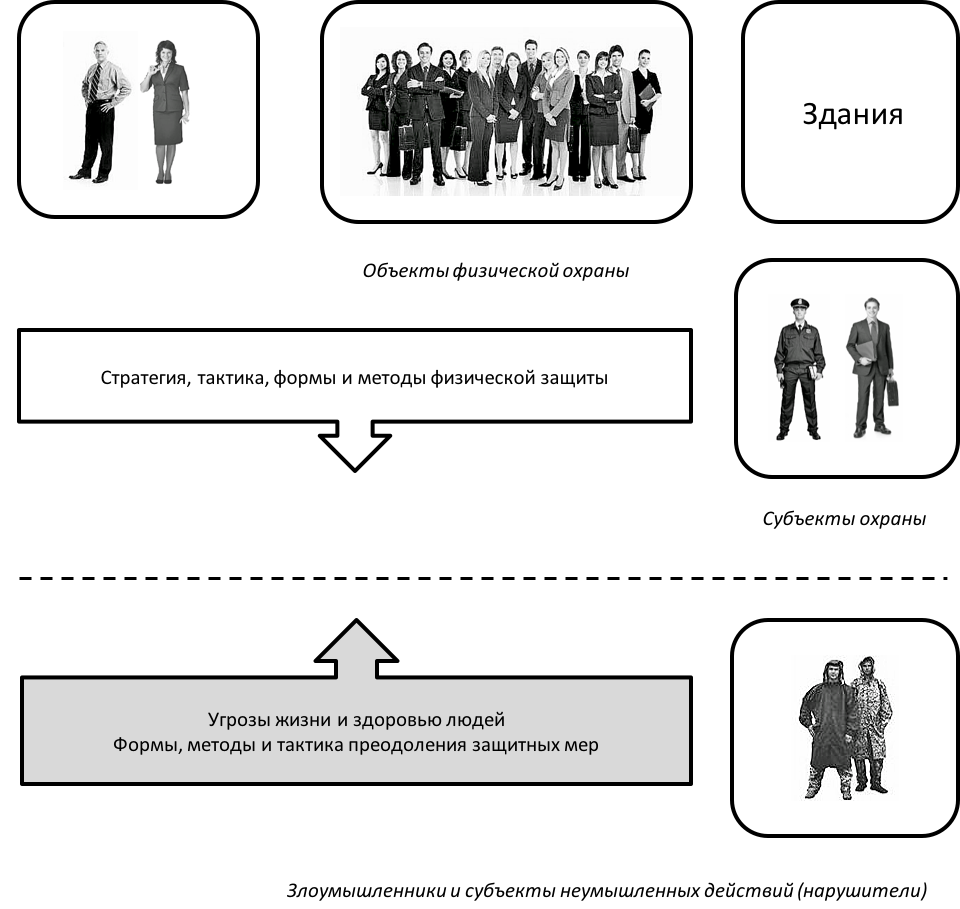
\includegraphics[scale=0.7]{img1}
	\caption{Угроза и защита в области обсепечения физической безопасности}
	\label{image1}
\end{figure}

К \textit{объектам физической охраны} относятся:
\begin{itemize}
	\item Собственники бизнеса и члены их семей;
	\item Топ-менеджеры и персонал предприятия, места их нахождения;
	\item Товарно-материальные и финансовые ценности;
	\item Служебная документация, составляющая коммерческую и иную тайну, а также объекты интеллектуальной собственности;
	\item Объекты недвижимости, а также объекты обеспечения жизнедеятельности предприятия (энергообеспечение, теплоснабжение, водоснабжение и др.).
\end{itemize}

Как правило, объектами физического насилия стано­вятся руководители предприятий или сотрудники, зани­мающие определенное должностное положение (принимают управленческие и кадровые решения, имеют право подписи финансовых документов, участвуют в пла­нировании работы предприятия, заключении сделок, ин­вестиционных проектах и пр.). Вместе с тем, отдельные сотрудники могут становиться объектами физических посягательств и в силу различных конфликтных ситуаций.\\

\begin{tcolorbox}[colback=blue!55!red!5!,colframe=blue!55!red,enforce breakable,% use only breakable in the real world!
	pad at break=1mm, title=Кейс 28. Действия обиженного сотрудника]
	
	7 ноября 2012 г. юрист Дмитрий Андреевич Виноградов, 1983 года рождения приехал на работу в компанию «Ригла» (г. Москва) с рюкзаком, в котором находилось специальное снаряжение и боеприпасы, и двумя ружейными чехлами, в которых находились карабины «Сайга» и «Benelli».
	
	В головном офисе фармацевтической компании он беспрепятственно прошел пост охраны, включая металлодетектор. Зашел в мужской туалет на 3-м этаже, где переоделся в военизированный костюм, расчехлил и подготовил к стрельбе оружие. По дороге с третьего на четвертый этаж Виноградов встретил случайно проходившего сотрудника компании и расстрелял его. Затем он прошел к кабинету № 400 и эффектно вошел туда с двумя карабинами наперевес, где начал расстреливать всех присутствовавших. На месте им было убито 4 человека (двое мужчин и две женщины). Двое тяжело раненных лиц были доставлены в клинику, где один из потерпевших скончался от полученных ранений в грудную клетку. Силами службы безопасности «Риглы» Виноградов был задержан и обезоружен. По предварительным данным следствия, он совершил преступление на почве неразделенной любви, а жертвами стали коллеги любимой девушки, которые иронично относились к чувствам Виноградова. К убийству нескольких человек преступник готовился практически год. В это время он не только купил длинноствольное оружие и посещал стрелковый клуб, но и обращался к психиатру с жалобой на проблемы с психикой. 
	
	Начальник охраны «Риглы» был уволен, но это не помогло вернуть к жизни погибших.

\begin{itemize}
	\item[{\color{blue!55!red}\Huge {  $ ? $}} \quad]   Сообщите свое мнение о том, как можно было предотвратить преступление.
\end{itemize}	
	
\end{tcolorbox}

В общем плане к угрозам физической безопасности личности относятся: 
\begin{itemize}
	\item Похищения и угрозы похищения сотрудников, членов их семей и близких родственников; 
	\item Убийства, сопровождаемые насилием, издевательствами и пытками; 
	\item Психологический террор, угрозы, запугивание, шантаж, вымогательство; 
	\item Нападение с целью завладения денежными средствами, ценностями и документами. 
\end{itemize}

Основными способами реализации указанных угроз, как правило,  являются следующие\footnote{Ворона В.А., Тихонов В.А. Концептуальные основы создания и применения системы защиты объектов. М.: Горячая линия – Телеком, 2012. С 28-29}:
 
\begin{itemize}
	\item Взрывы, в том числе с использованием взрывных ус­тройств, снабженных механизмами дистанционного уп­равления; 
	\item Обстрелы  из автоматического  оружия различных калибров, в том числе с использованием специальных при­способлений для ведения снайперской стрельбы в любое время суток; 
	\item Поджоги, в том числе с использованием канистр и иных емкостей с легко воспламеняющимися жидкостями и смесями; 
	\item Акты вандализма, повреждение входных дверей, ре­шеток, ограждений, витрин, а также личных и служебных транспортных средств; 
	\item Ограбления   и   разбойные   нападения   на   офисы, склады и транспортные средства,  перевозящие ценные грузы; 
	\item Налеты на квартиры руководителей компаний или сотрудников фирм; 
	\item Умышленные и заказные убийства; 
	\item Захват заложников; 
	\item Физическое насилие в отношении отдельных со­трудников фирм или членов их семей;
	\item Шантаж, угрозы физического насилия или убий­ства. 
\end{itemize}

В качестве основных мер обеспечения физической безопасности объектовая охрана, организация внутриобъектового и пропускного режимов, мониторинг внешней и внутренней среды охраняемого объекта, личное сопровождение охраняемых лиц, обеспечение режима конфиденциальности маршрутов их передвижения, конкретных мест посещения и мест жительства, отработка стандартных и проверочных маршрутов при передвижении охраняемых лиц.\\

\begin{tcolorbox}[colback=blue!55!red!5!,colframe=blue!55!red,enforce breakable,% use only breakable in the real world!
	pad at break=1mm, title=Кейс 29. Инциденты при охране физических лиц]

	30 марта 1981 г. президент США Рональд Рейган вышел из гостиницы «Хилтон» и направился в сторону ожидавшей его автомашины. В это время из толпы вышел Джон Хинкли, выхватил револьвер и, удерживая оружие двумя руками, направил его на президента. Охрана среагировала мгновенно. Один из телохранителей бросился на преступника и сбил его с ног еще до того, как Хинкли успел выстрелить первый раз. До того, как успел нажать на спусковой крючок! А ведь это был выстрел в упор. Другой телохранитель, прикрывая своим телом президента, сгреб его в охапку и втолкнул в бронированный лимузин. Все это заняло менее трех секунд. Однако душевнобольной Хинкли оказался неплохим стрелком. За три секунды в падении он сумел сделать шесть выстрелов. Только последняя пуля попала в автомобиль и рикошетом - в грудь Рейгана! Семидесятилетний президент США остался жив благодаря опыту и самоотверженности личных телохранителей, оказавшихся эффективными на последнем рубеже защиты охраняемого лица. 
	
	28 сентября 2012 г. во время праздничного мероприятия по случаю открытия моста в Храставе на Либерецах к проходившему в толпе президенту Чехии Вацлаву Клаусу приблизился молодой человек в защитном полувоенном костюме. Он достал из кармана пистолет и произвел в упор несколько имитационных выстрелов в правую руку и бок президента. Все произошло настолько быстро, что никто не смог помешать нападавшему. Стрелявший повернулся и спокойно ушел с места происшествия. Телохранители Вацлава Клауса не только отстали на маршруте от охраняемого лица, но и, как оказалось, просто были не готовы к действиям в данной ситуации. Никто не смог задержать покушавшегося и даже не попытался это сделать. Нападавшим оказался 26-летний местный рабочий Павел Вондроуш. Перед задержанием он еще успел спокойно выкурить сигарету и дать интервью подоспевшим журналистам. Свой поступок он объяснил как протест против политиков, которые не замечают простой народ. Намерений навредить Клаусу у него, якобы, не было, т.к. пистолет был игровым. Однако у президента от выстрелов пластиковыми пулями остались синяки, а рубашка оказалась испачкана кровью. Комиссия констатировала, что со стороны охраны имел место профессиональный провал, полное фиаско. Начальник охраны Иржи Скленка подал в отставку.

\begin{itemize}
	\item[{\color{blue!55!red}\Huge {  $ ? $}} \quad]   Проведите сопоставительный анализ действий охраны президентов США и Чехии.
\end{itemize}	

\end{tcolorbox}

Личная охрана должна соответствовать образу жизни охраняемого лица, отличаться решительностью, эффективностью и не броскостью, быть хорошо информированной и уметь хранить конфиденциальную информацию. Сотрудники личной охраны должны быть профессионалами, во время работы не отвлекаться на сторонние вопросы и действовать на упреждение. Своим поведением они не должны давать повода для агрессии. В критических ситуациях сотрудники личной охраны должны быть готовы к самопожертвованию. Руководители охраны обязаны знать, что профессиональные киллеры составляют досье на объекта покушения, изучают маршруты передвижения, места жительства и работы на уязвимость, определяют места и способы покушений.

В целях предупреждения совершения противоправных действий на объектах, специалисты рекомендуют категорировать их на \textit{особо важные, особо режимные, режимные} и \textit{не режимные объекты}. Внутри объекта, в зависимости от его категории, рекомендуют выделять несколько зон безопасности (см. рисунок \ref{image2}). В каждой из указанных на рисунке зон устанавливается свой режим безопасности, связанный с особенностями мер по разграничению доступа сотрудников предприятия и сторонних посетителей. Как правило, в зонах устанавливаются предназначенные для них специальные технические средства. В отдельных зонах комплексно применяют физическую охрану и технические средства. Иногда на периферии устанавливается контрольное оборудование, а управление им осуществляется людьми из центра мониторинга.

\begin{figure}[h]
	\centering
	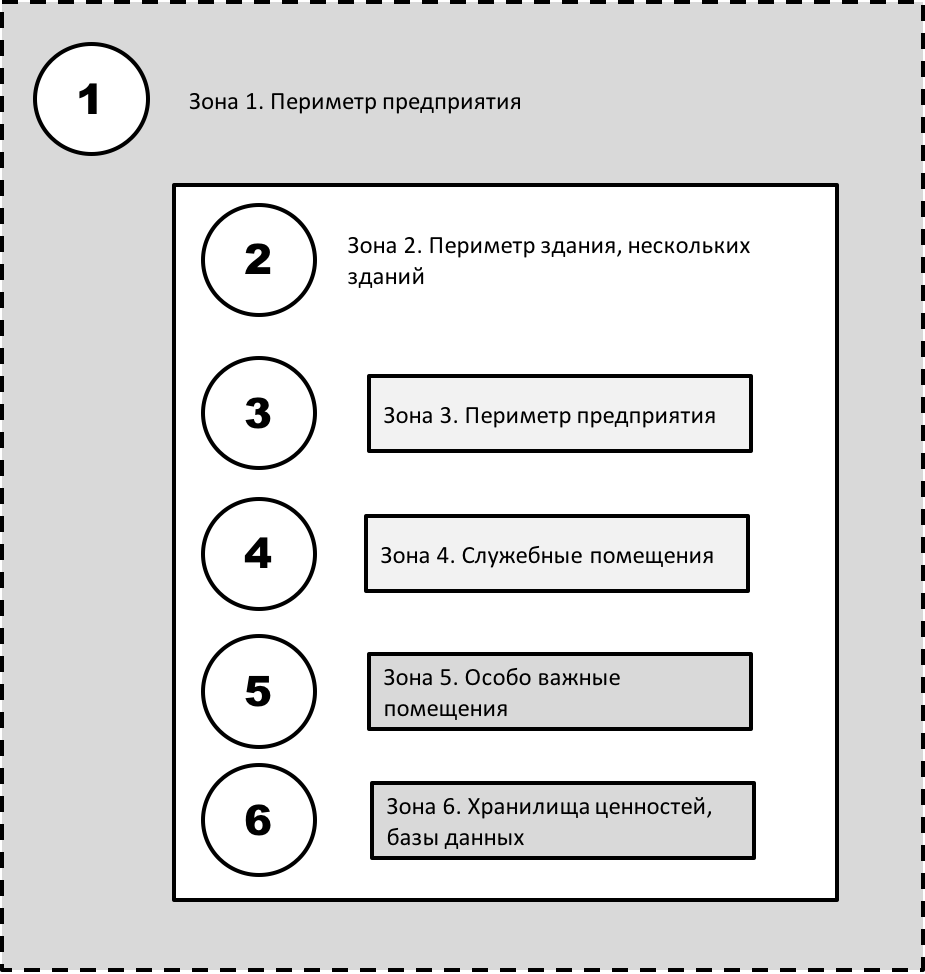
\includegraphics[scale=0.6]{img2}
	\caption{Зоны безопасности внутри объекта по В.А. Вороне и В.А. Тихонову}
	\label{image2}
\end{figure}

В качестве основных \textit{групп причин угроз безопасности личности}, как правило, указывают следующие:
\begin{itemize}
	\item Недобросовестная конкуренция (устранение конкурента);
	\item Действия криминальных сообществ, организаций и преступных групп; 
	\item Попытки добропорядочных граждан решать свои экономические проблемы за счет богатых друзей, знакомых и родственников;
	\item Противоправное урегулирование финансовых конфликтов (расправы с ненадежными партнерами, неплательщиками крупных долгов, устранение кредиторов);
	\item Сокрытие фактов коррупции, устранение свидетелей других преступных действий.
\end{itemize}

\subsection{Угроза сохранности финансов и иных материальных ценностей предприятия}

Субъекты предпринимательской деятельности осуществляют операции с наличными и безналичными денежными средствами, иными материальными ценностями. Данные средства, обладающие существенным стоимостным выражением, бывают представлены в виде: 
\begin{itemize}
	\item Российской и иностранной наличной и безналичной валюты; ценных бумаг; 
	\item Подлинников правоустанавливающих документов; драгоценных и полудрагоценных камней;
	\item Драгоценных металлов и изделий из камней и металлов;
	\item Дорогостоящего движимого имущества; 
	\item Произведений искусства, антикварных ценностей и др. 
\end{itemize}
	
Указанные предметы и документы всегда являлись объектом покушения злоумышленников и, в этой связи, всегда охранялись (см. рисунок \ref{image3}).

С учетом того, что материальные и иные ценности носят разный характер, а также выполняют различные функции на различных этапах производства, злоумышленники вырабатывают различные методы завладения защищаемыми объектами, а физическая охрана постоянно совершенствует меры защиты. К примеру, драгоценные металлы и камни являются объектами четко регламентированной физической защиты на всех этапах производственной цепочки: добыча (производство), обогащение, обработка (включая огранку), производство продукции для целей науки, техники и личного потребления. Это делается осознанно – на всех стадиях драгоценные металлы и камни являются объектами преступных посягательств. Субъектами противоправной деятельности могут быть сторонние лица, работники предприятий отрасли и даже работники охраны. По этой причине защитные меры должны носить комплексный характер, быть сбалансированными и предусматривать применение принципа «не менее двух ключей».

В отрасли по добыче и переработке природных нефти и газа также на всех этапах технологической цепочки сложились традиционные методы хищения энергоносителей. Как правило, наибольшие объемы незаконного отъема совершаются в процессе перекачки нефти и газа по трубопроводным магистралям. К примеру, сразу после распада Советского Союза в 1991 г., украинские юридические лица приступили к несанкционированному отбору (хищению) газа, поступавшего из России транзитом через территорию Украины в страны западной Европы. Злоумышленники использовали особенность конструкции трубопроводных систем в рамках единой страны (СССР), что не позволяло с территории Российской Федерации в полной мере контролировать действия компании «Укртрансгаз» и связанных с ней должностных лиц. 

\begin{figure}[h]
	\centering
	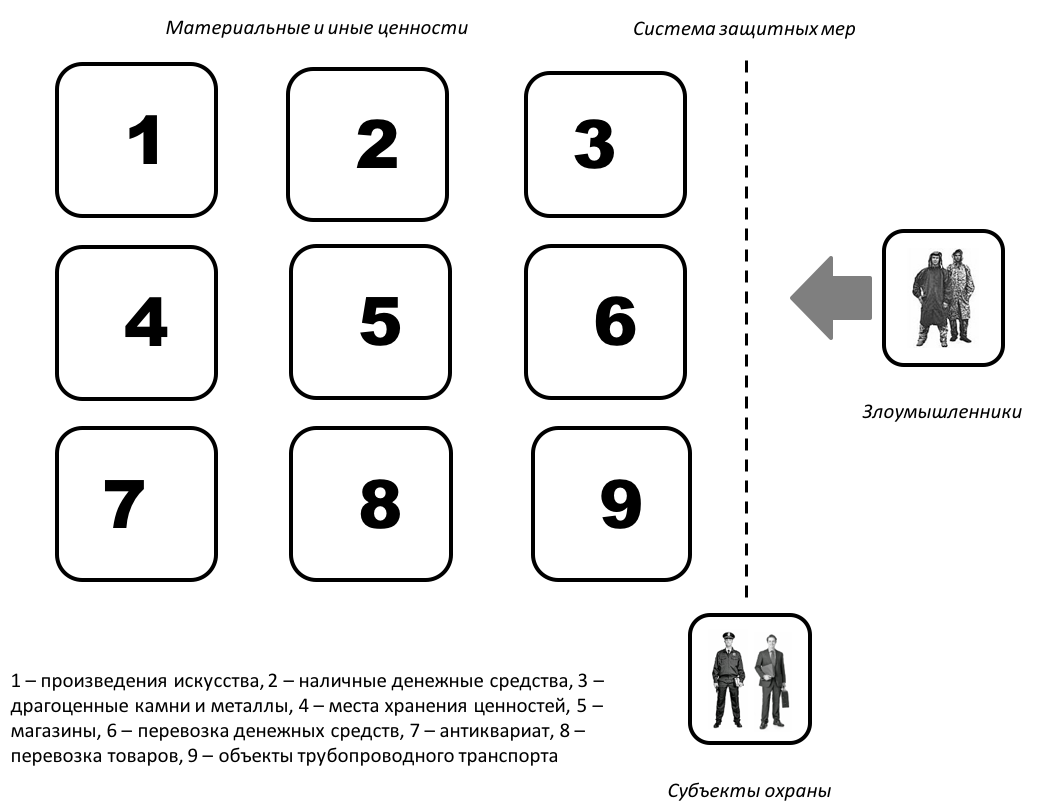
\includegraphics[scale=0.7]{img3}
	\caption{Принципиальная схема физической зашиты ценностей откорыстных посягательств}
	\label{image3}
\end{figure}

На объектах трубопроводного транспорта, связанных, прежде всего, с перекачкой нефти, нефтепродуктов и природного газа, распространенным явлением является хищение путем несанкционированной врезки в магистральный трубопровод. При этом в последнее время наиболее часто подобный метод используется в удаленных местностях, путем осуществления врезки под землей и под водой, с другими ухищрениями, осложняющими поиск и выявление неправомерных действий злоумышленников.

Основные угрозы сохранности материальных ценностей предприятия реализуются, как правило, в следующих основных формах:
\begin{itemize}
	\item Деятельность преступных групп, конкурирующих экономических структур, а также отдельных лиц, занимающихся противоправными действиями в отношении собственности, которые могут привести к значительным материальным и финансовым потерям организации или ее отдельным подразделениям.
	\item Непреднамеренные (ошибочные, случайные, необдуманные, без корыстных целей) нарушения установленных требований учета, хранения, оборота, правил торговли товарно-материальных ценностей, финансовых ресурсов, служебных документов и информации, приводящие к непроизводительным затратам ресурсов, утратам и хищениям.
	\item Преднамеренные (в корыстных целях, по принуждению, со злым умыслом, т.п.) действия сотрудников компании, допущенных к материальным, финансовым и информационным ресурсам:
	\begin{itemize}
		\item Различные виды хищений товарно-материальных ценностей отдельными сотрудниками или в сговоре на объектах организации;
		\item Умышленное нарушение денежно-кассовых операций с клиентами, поставщиками продукции, повлекшее недостачи;   
		\item Подделка учетных и отчетных документов хранения и оборота товарно-материальных ценностей;
		\item Хищение носителей конфиденциальной информации (распечаток, магнитных дисков, запоминающих устройств) для использования в личных корыстных целях.
	\end{itemize}
	\item Отказы и сбои в работе инженерно-технических средств охраны (систем СКУД, ОПС, видеонаблюдения и связи), приводящие к непроизводительным затратам:
	\begin{itemize}
		\item отключение электричества в офисе и на объектах предприятия;
		\item незапланированная потеря каналов связи, невозможность управления системой охранно-пожарной сигнализации и видеонаблюдения на объектах с пульта централизованного наблюдения;
		\item нарушение функционирования пульта централизованного наблюдения у оперативного дежурного (некомпетентность оператора, сбой программного обеспечения, выход из строя отдельных комплектующих компьютера, др.);
		\item выход из строя системы видеонаблюдения на объектах компании, вследствие чего допущены непроизводственные потери материальных и финансовых средств;
		\item нарушение работы системы СКУД, несанкционированный пропуск посторонних лиц на территорию объектов компании, допуск к товарно-материальным ценностям, конфиденциальной информации.
	\end{itemize}
	\item Аварии, техногенные катастрофы и природные катаклизмы.
\end{itemize}

Отдельную сферу угроз финансовым и материальным ценностям составляют угрозы в сфере инкассации. Они также носят как внешний, так и внутренний характер. Инкассация является специализированной сферой банковской деятельности и по этой причине лицензируется Банком России и его территориальными учреждениями. С другой стороны, инкассация выражается в перемещении наличных денежных средств и иных материальных ценностей под охраной. По этой причине в своей деятельности инкассация использует оружие, боеприпасы и специальные средства.  Одной из важнейших внутренних задач является обеспечение кадровой безопасности службы инкассации.\\


\begin{tcolorbox}[colback=blue!55!red!5!,colframe=blue!55!red,enforce breakable,% use only breakable in the real world!
	pad at break=1mm, title=Кейс 30. Чрезвычайное происшествие в Перми]
	
	29 июня 2009 г. в Перми было совершено разбойное нападение на автомобиль инкассации Западно-Уральского банка ОАО «Сбербанк России». В результате данного преступления было похищено 250 000 000 руб. наличными\footnote{Сайт «Википедия» [Электронный ресурс], информационно-справочный портал. М. URL: https: //ru.wikipedia.org (дата обращения: 24.02.2015 г.)}. По факту было возбуждено уголовное дело и начаты оперативно-розыскные мероприятия. В результате было установлено, что автомашина инкассации с крупной суммой наличных денежных средств направлялась в рассчетно-кассовый центр банка. Старший инкассатор Шуман А.В., угрожая огнестрельным оружием своим коллегам, заставил их заехать вглубь лесного массива и остановить там автомобиль. После этого злоумышленник запер инкассаторов в бронированной кабине автомобиля и перегрузил мешки с деньгами в поджидавший его легковой автомобиль и скрылся в неизвестном направлении. Принятыми мерами Шуман А.В. и другие участники преступной группы были обнаружены и задержаны. Организатор преступления указал на место нахождения тайника с похищенными деньгами. В банк была возвращена практически вся сумма, исключением 1 145 000, 300 руб. уже потраченных преступниками. Во время следствия было установлено, что Шуман А.В. более 12 лет работал инкассатором и был на хорошем счету. К преступлению он готовился два года. В качестве побуждающего мотива бывший инкассатор сослался на сложную, опасную и мало оплачиваемую работу. 10 февраля 2010 г. судом Шуман А.В. был признан виновным в совершении ограбления и приговорен к восьми годам лишения свободы в исправительной колонии строгого режима. Трое соучастников описанного преступления были также привлечены к уголовной ответственности.	

\begin{itemize}
	\item[{\color{blue!55!red}\Huge {  $ ? $}} \quad]   Предложите меры по предотвращению корыстных преступлений со стороны инкассаторов.
\end{itemize}	
	
\end{tcolorbox}
	
Еще больше рисков возникает при инкассации ценностей не уполномоченными на то лицами. «Серые» схемы инкассации производятся с участием частных охранных предприятий и даже работников полиции, которые не имеют соответствующей лицензии Банка России. В ряде случаев подобные бригады инкассаторов имеют даже табельное оружие, однако они не имеют необходимой профессиональной подготовки и часто становятся жертвами нападений преступников. В некоторых организациях допускаются «черные» схемы инкассации, когда в качестве курьеров для перевозки денежных средств используются собственные штатные работники – бухгалтера и водители. Руководители предприятий, которые таким образом пытаются минимизировать расходы. В ряде случаев это приводит не только к безвозвратной потере крупных сумм денежных средств, но и к гибели людей, давших согласие эти средства перевозить. Отдельные работники коммерческих банков даже пытаются путем нарушения правил совершения валютно-денежных операций и правил инкассации, разрабатывать схемы зарабатывания средств на обменных операциях, игнорируя всевозможные угрозы. В таких ситуациях к операционным искам добавляются риски контрагентов и весьма реальные риски потери деловой репутации.\\
	
\begin{tcolorbox}[colback=blue!55!red!5!,colframe=blue!55!red,enforce breakable,% use only breakable in the real world!
	pad at break=1mm, title=Кейс 31. Изобретательный менеджер]

	20 сентября 1999 г. коммерческий банк «Первое общество взаимного кредита» в процессе совершения валютно-обменной операции утратил наличные денежные средства в сумме свыше 250 000 долларов США. Проведенное по факту служебное расследование позволило установить, что материальный ущерб банку был нанесен в результате действий первого заместителя председателя правления данного финансового учреждения, которого мы назовем «Першин». Неправильно трактуя свои должностные полномочия и игнорируя требования действующего законодательства, руководитель на регулярной основе осуществлял «черные схемы» валютно-обменных операций. Каждое утро «Першин» лично обзванивал пункты обмена валюты столичного города и составлял схему из нескольких операций в целях получения определенной прибыли от каждой. После этого по его указанию из хранилища банка изымали часть наличных денежных средств, их складывали в личные автомобили работников казначейства банка, которые объезжали несколько обменных пунктов. При этом сотрудники казначейства, боясь потерять работу, шли на выполнение поручений, но перед выездом даже прощались с коллегами, понимая рискованность ситуации. При совершении последней операции они передали 250 000 долларов «кассиру» обменного пункта, который закрыл шторку окна под предлогом пересчета. Работники банка прождали около часа, стали стучаться в окно пункта и, в конечном итоге, установили, что работники обменного пункта исчезли вместе с деньгами. Служебное расследование также показало, что по указанию «Першина» было проведено более 20 подобных операций, прибыль от которых в общем итоге составила 74 тыс. рублей. Последняя операция нанесла ущерб банку, перекрыв на несколько порядков полученный ранее сомнительный доход.	
	
\begin{itemize}
	\item[{\color{blue!55!red}\Huge {  $ ? $}} \quad]   Опишите банковские нормативы, которые возможно были нарушены менеджером.
\end{itemize}	
	
\end{tcolorbox}	
	
	
\subsection{Угроза сохранности объектов недвижимости}	
	
Здания, сооружения и иное недвижимое имущество относятся к основным средствам предприятия. Как правило, они являются дорогостоящими объектами собственности, требующими постоянного вложения средств в текущие и капитальные ремонты, переоборудование. Недвижимость также подлежит страхованию, и она же является объектом налогообложения. В то же время недвижимость может быть гарантией внешних обязательств предприятия, считается «твердым» залогом при получении кредитов, является подтверждением реальной производственной деятельности.

Естественно, что объекты недвижимости подвержены рискам. Некоторые из них носят объективный характер – природоестественные, техногенные и экологические катастрофы, неблагоприятные политические факторы, включая масштабные войны и локальные вооруженные конфликты. Многие риски связаны с умышленными или неумышленными действиями людей и носят субъективный характер. Тем не менее, подобные конфликты также могут нанести существенный ущерб. Любое предприятие, владеющее объектами недвижимости, должно умело защищать их от рисков (см. рисунок \ref{image4}).

\begin{figure}[h]
	\centering
	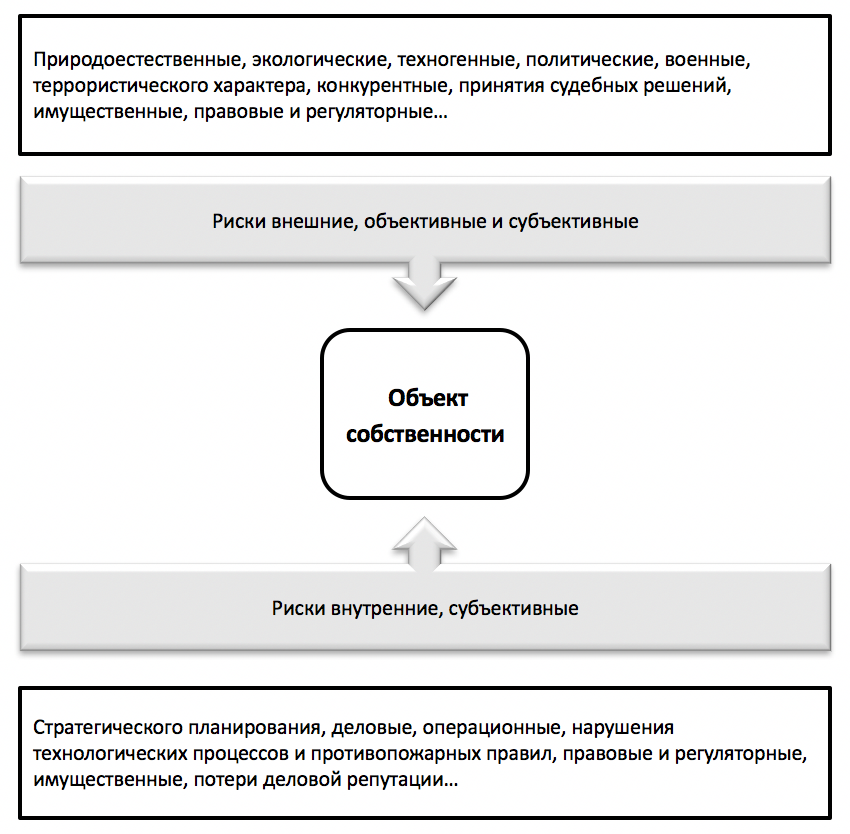
\includegraphics[scale=0.7]{img4}
	\caption{Риски и угрозы сохранности объектов собственности}
	\label{image4}
\end{figure}

Как следует из размещенного выше рисунка, риски сохранности объектов недвижимости могут быть внешними и внутренними, могут носить объективный и субъективный характер. Часть внешних рисков может минимизироваться путем страхования и перестрахования имущества. Однако возможную реализацию некоторых рисков этой категории сложно спрогнозировать заранее. К примеру, весной 2013 г. сложно было предположить, что на Украине произойдет государственный переворот, который повлечет за собой смену власти, силовой передел собственности, локальные вооруженные конфликты, повлекшие за собой массовую гибель людей, уничтожение промышленных объектов и инфраструктуры.

С учетом этих особенностей преступные посягательства на здания и помещения в отдельных регионах из категории потенциальных рисков переходят в категорию рисков реальных, угроза возникновения которых становится весьма вероятной:
\begin{itemize}
	\item Взрывов;
	\item Обстрелов из огнестрельного оружия;
	минирования, в том числе с применением дистанционного управления;
	\item Поджогов;
	\item Нападения, вторжения, захватов, пикетирования, блокирования;
	\item Повреждения входных дверей, решеток, ограждений, витрин, мебели, а также транспортных средств личных и служебных;
	\item Технологические аварии, пожары.
\end{itemize}

Целями подобных акций могут быть нанесение серьезного материального и морального ущерба, срыв на длительное время нормального функционирования объектов, вымогательство значительных сумм денег или каких-либо льгот (кредиты, отсрочка или погашение платежей и т. п.) перед лицом террористической угрозы. В зонах локальных вооруженных конфликтов такие цели могут быть вызваны исключительно военными соображениями. По мнению некоторых специалистов\footnote{Люттвак Э.Н. Стратегия: логика войны и мира. М.: Университет Дмитрия Пожарского, 2012. С 149}, чем сильнее акцент на истощение противника в общем стиле войны, тем эффективнее становятся техники обнаружения цели, атаки и снабжения. Такой процесс заменяет собой искусство войны. Всякий раз, когда материально превосходящая сторона способна извергать боевую мощь, она без ограничения наносит удары на позиции противника (окопы, города и иные населенные пункты, объекты промышленности и социальной сферы).

В любом случае следует учитывать, что ряд объектов недвижимости нуждается в повышенных мерах физической защиты от любых внешних и внутренних угроз. К таким особо важным и важным объектам можно отнести предприятия по изготовлению боеприпасов, высокотоксичные производства, объекты атомной энергетики, гидротехнические сооружения, объекты добычи, транспортировки и переработки нефти и газа, места хранения значительных материальных ценностей. Указанные и некоторые другие объекты нормативно категорированы и отнесены к области государственного мониторинга по вопросам противопожарной защиты, гражданской обороны и комплексного обеспечения их безопасности. Физическая охрана таких, равно как и иных объектов может быть отнесена к компетенции различных охранных структур, деятельность которых разрешена в нашей стране.\\	

\begin{tcolorbox}[colback=blue!40!red!1!,colframe=blue!40!red,enforce breakable,% use only breakable in the real world!
	pad at break=1mm, title=Вопросы и задания для самоконтроля]
	\begin{itemize}
		\item[{\color{blue!55!red}\Huge { $ ? $}} ]  Дайте определение понятия «частная охранная деятельность».
		\item[{\color{blue!55!red}\Huge {  $ ? $}} ] Опишите возможные угрозы в области защиты жизни и здоровья физических лиц.
		\item[{\color{blue!55!red}\Huge {  $ ? $}} ] Расскажите об угрозах проникновения посторонних лиц в места хранения материальных ценностей.
		\item[{\color{blue!55!red}\Huge {  $ ? $}} ] Расскажите об угрозах проникновения на охраняемые объекты посторонних лиц, представляющих интересы рейдеров.
		\item[{\color{blue!55!red}\Huge {  $ ? $}} ] Расскажите об угрозах похищения наличных денежных средств и иных материальных ценностей во время их инкассации.		
	\end{itemize}		
\end{tcolorbox}

\section{Организация частной и иной охранной деятельности}

\begin{tcolorbox}[colback=blue!40!red!10!,colframe=blue!40!red]
В результате изучения главы студент должен \textbf{знать} субъектов осуществления различных видов обеспечения физической безопасности в нашей стране, их полномочиях, права и обязанности; \textbf{уметь} выделять особенности организации деятельности ведомственной охраны предприятий и организаций, частных охранных предприятий и военно-охранных компаний, вневедомственной охраны полиции и порядком осуществления государственной охраны высших должностных лиц страны; \textbf{владеть} методами применения на предприятии физической охраны, подходами определения ее состава и направлений взаимодействия внутри системы безопасности, а также расчета экономических затрат на применение различных вариантов физической защиты.
\end{tcolorbox}

\subsection{Порядок создания и функционирования частных охранных предприятия}

В соответствии с действующим законодательством охранную деятельность в нашей стране осуществляют федеральные государственные органы, специально выделенные структурные подразделения министерств, ведомств, организаций и предприятий. Каждый из участников этой деятельности обладает своей сферой компетенции и установленными полномочиями. Ряд указанных структур, а также организации с особыми уставными задачами наделены правом на хранение и применение оружия, патронов к нему и специальных средств. Общую структуру и взаимосвязь государственных органов и иных организаций, осуществляющих охранную деятельность в Российской Федерации, можно представить следующим образом (см. рисунок \ref{image5}). Как правило, функции охранных структур разграничены, однако в ряде случаев некоторые государственные и частные организации конкурируют на рынке услуг безопасности.

\begin{figure}[h]
	\centering
	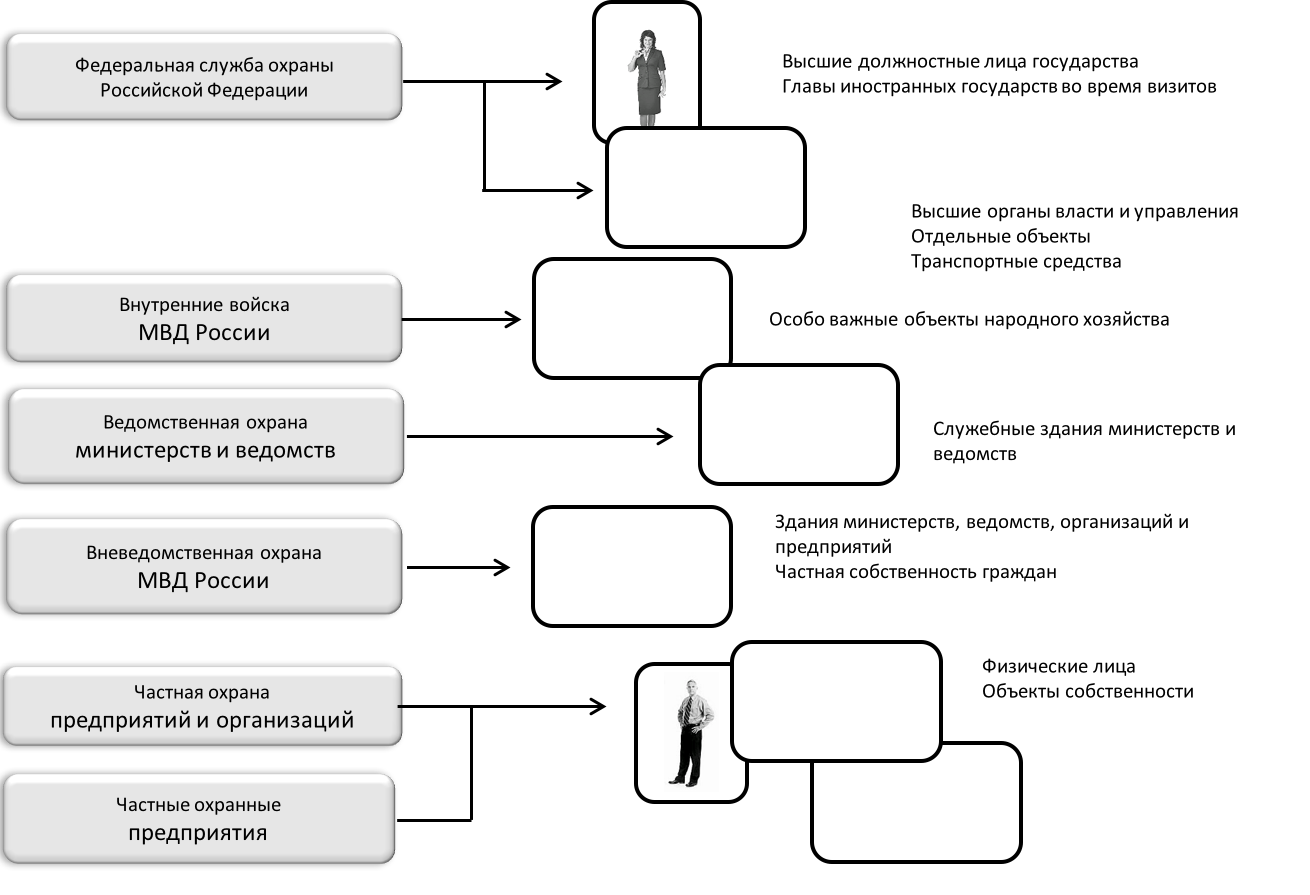
\includegraphics[scale=0.7]{img5}
	\caption{Органы, предприятия и организации, наделенные правом осуществления функция охраны}
	\label{image5}
\end{figure}

Частная охранная деятельность в нашей стране регулируется федеральным законодательством с 1992 г. Соответствующий федеральный закон имеет прямое действие. \\

\definition{Частная охранная деятельность}{оказание на возмездной договорной основе услуг физическим и юридическим лицам имеющими специальное разрешение (лицензию) органов внутренних дел организациями и индивидуальными предпринимателями в целях защиты законных прав и интересов своих клиентов.}

В целях охраны разрешается предоставление следующих услуг:
\begin{itemize}
	\item Защита жизни и здоровья граждан;
	\item Охрана объектов и (или) имущества (в т.ч. при его транспортировке), находящихся в собственности, во владении, в пользовании, хозяйственном ведении, оперативном управлении или доверительном управлении, за некоторыми исключениями;
	\item Охрана объектов и (или) имущества на объектах с осуществлением работ по проектированию, монтажу и эксплуатационному обслуживанию технических средств охраны, перечень видов который устанавливается Правительством Российской Федерации, и (или) с принятием соответствующих мер реагирования на их сигнальную информацию;
	\item Консультирование и подготовка рекомендаций клиентам по вопросам правомерной защиты от противоправных посягательств;
	\item Обеспечение порядка в местах проведения массовых мероприятий;
	\item Обеспечение внутриобъектового и пропускного режимов на объектах;
	\item Охрана объектов и (или) имущества, а также обеспечение внутриобъектового и пропускного режимов на объектах, в отношении которых установлены обязательные для выполнения требования к антитеррористической защищенности, за исключением объектов, подлежащих государственной охране.
\end{itemize}

Как было указано выше, частная охранная деятельность не распространяется на объекты государственной охраны, а также некоторые иные охраняемые объекты, перечень которых утверждается Правительством Российской Федерации. Запрещается вооруженная охрана имущества на территориях закрытых административно-территориальных образований, а также приобретение и использование оружия частными охранными организациями, зарегистрированными и (или) расположенными на их территориях. Оказание охранных услуг в целях защиты объектов транспортной инфраструктуры и транспортных средств от актов незаконного вмешательства осуществляется с учетом требований законодательства о транспортной безопасности.

Право на приобретение правового статуса частного охранника предоставляется гражданам, прошедшим профессиональное обучение для работы в данном качестве и сдавшим квалификационный экзамен. Статус подтверждается выдачей удостоверения частного охранника. Не вправе претендовать на статус частного охранника лица:
\begin{itemize}
	\item Не достигшие восемнадцати лет; признанные решением суда недееспособными или ограниченно дееспособными;
	\item Имеющие заболевания, которые препятствуют исполнению ими обязанностей частного охранника (перечень таких заболеваний устанавливается Правительством Российской Федерации);
	\item Имеющие судимость за совершение умышленного преступления; 
	\item Которым предъявлено обвинение в совершении преступления; 
	\item А также лица, в отношении которых по результатам проверки имеется заключение о невозможности допуска к осуществлению частной охранной деятельности в связи с повышенной опасностью нарушения прав и свобод граждан, возникновением угрозы общественной безопасности. 
	\item К работе частными охранниками также не допускаются лица, досрочно прекратившие полномочия по государственной должности или уволенные с государственной службы, в т.ч. из правоохранительных органов, из органов прокуратуры, судебных органов по основаниям совершения ими дисциплинарных проступков, грубым или систематическим нарушениям дисциплины, совершением проступка, порочащего честь государственного служащего, утратой доверия к нему, если с момента прекращения полномочий (увольнения) прошло менее трех лет. 
\end{itemize}

Уполномоченным органом в области лицензирования частной охранной деятельности являются органы внутренних дел. В МВД России эту деятельность координирует Управление по организации лицензионно-разрешительной работы и соответствующие подразделения территориальных органов. Им предоставлены полномочия по оказанию следующих государственных услуг\footnote{Официальный сайт Министерства внутренних дел Российской Федерации. Управление по организации лицензионно-разрешительной работы [Электронный ресурс] //mvd.ru: информационно-справочный портал. М. URL: https://mvd.ru/mvd/structur1/Upravleni/ulrr/Gosv (дата обращения: 26.02.2015)}:

\begin{itemize}
	\item Прием квалификационного экзамена у граждан, прошедших ранее обучение по программе профессиональной подготовки частных охранников;
	\item Выдача лицензии на частную охранную деятельность;
	\item Выдача удостоверения частного охранника;
	\item Исполнение функции контроля за частной охранной деятельностью;
	\item Выдача юридическим лицам с особыми уставными задачами разрешения на хранение и использование служебного оружия и патронов к нему.
\end{itemize}

В рамках охранного бизнеса первоначально оформляется лицензия юридического лица на право заниматься частной охранной деятельностью. На следующем этапе устанавливается и изучается объект охраны, формируется концепция его защиты, производится расчет требуемых сил и средств, набирается персонал охраны.

Первоначально, чтобы не терять динамики, можно набирать на работу уже лицензированный персонал. В последующем можно сделать акцент на подборе кадров в соответствии с собственными критериями, а в последующем направить их на обучение в одно из специализированных учебных заведений. После обучения слушатели должны будут сдать квалификационный экзамен в органах внутренних дел и получить удостоверение частного охранника. Только эти лица получат право на ношение и применение служебного оружия. Пакет документов для получения лицензии в обязательном порядке должен включать: медицинскую справку о состоянии здоровья; документы, подтверждающие прохождение специальной подготовки для работы в качестве частного охранника; или стаж работы в органах внутренних дел, органах безопасности не менее трех лет, а также сведения о потребности в специальных средствах, средствах связи и иных технических средствах, и намерении их использовать.

Стоимость охранных услуг бывает различной и зависит от ряда факторов. Прежде всего, она зависит от региона. В регионе стоимость охраны отличается в крупных городах, небольших населенных пунктах, в зависимости от категории охраняемого объекта, а также определяется количеством постов охраны и их вооруженностью.\\

\begin{tcolorbox}[colback=blue!55!red!5!,colframe=blue!55!red,enforce breakable,% use only breakable in the real world!
	pad at break=1mm, title=Кейс 32. Стоимость охранных услуг]
	
	Как правило, стоимость охранных услуг указана на сайтах охранных предприятий. К примеру, группа частных охранных предприятий «Бастион» подробно изложила стоимость своих услуг в пересчете за один круглосуточный пост: от 70 тыс. руб. в месяц (строительные площадки), от 85 тыс. руб. в месяц (магазины, торговые и офисные центры, коттеджные поселки, ТСЖ); от 120 тыс. руб. в месяц (банки, визовые центры, гостиницы и рестораны). Группа частных охранных предприятий «Премьер» проводит дифференциацию стоимости охраны в зависимости от наличия или отсутствия оружия у охраны. Так один двухсменный пост в месяц в виде направления охранников вахтовым методом без оружия оценивается в 80 тыс. руб.; трехсменный пост без охраны – 96 тыс. руб.; а двухсменный пост с оружием – 115 тыс. руб. Случается и так: ЧОП «СТС Безопасность» и группа частных охранных компаний «Taggerd» не указывают стоимость своих услуг со ссылкой на индивидуальную договоренность с клиентом.	
	
	\begin{itemize}
		\item[{\color{blue!55!red}\Huge {  $ ? $}} \quad]   Предложите принципы отбора охранной компании.
	\end{itemize}	
	
\end{tcolorbox}

Значительно возрастают затраты на охрану в том случае, если планируется организация нескольких круглосуточных вооруженных постов, оборудование оружейной комнаты, организация дежурной части охраны (пульта мониторинга), оборудование технических средств безопасности с выводом на пульт централизованной охраны (ПЦО) вневедомственной охраны МВД, закупка форменной одежды охранников и специального снаряжения, средств радиосвязи, бронежилетов и пр.

\subsection{Порядок создания и функционирования частных военно-охранных компаний}

В последние годы наблюдается рост случаев участия частных охранных вооруженных формирований и компаний по обеспечению безопасности в конфликтных ситуациях. Так, за последние 20 лет, в основном в США и Великобритании, резко увеличилось число таких компаний, которые предоставляют свои услуги в зонах вооруженных конфликтов за рубежом и постконфликтных ситуациях. Только в Ираке насчитывается около 50 тысяч частных охранников - иностранцев.
	
Практика свидетельствует, что часто частные военно-охранные компании выполняют задачи военного или полувоенного характера. Деятельность таких компаний в ряде случаев сопровождается нарушением прав человека. Лица, завербованные такими компаниями, действуют в «серой зоне» в условиях ограниченного надзора или армейского контроля. В целом, создание частных армий – феномен далеко не новый. В наше время наблюдается беспрецедентное увеличение спроса на услуги частных военных и охранных компаний. Главную причину растущей популярности частных охранных предприятий следует искать в глобализации, в трансформации мировой экономической системы. Современные транснациональные корпорации, располагающие миллиардами долларов, нуждаются в защите своих интересов ничуть не меньше, чем государства.  

Теперь частные военные охранные компании либо являются подразделением огромных транснациональных компаний, либо организованы с помощью, и по заданию спецслужб. Например, в Ираке квалифицированные военные специалисты получают более 1000 долларов в день. В 2006 году в мире насчитывалось более 3 тыс. частных военных компаний, которые оперировали более, чем в 100 странах мира, на всех континентах, кроме Антарктиды. Их годовой оборот достигает \$100 млрд. В связи с продолжающейся войной в Афганистане и Ираке объем этого рынка продолжает расти. За период с 1994 по 2005 годы Министерство обороны США заплатило частным военно-охранным компаниям (только американским) более \$400 млрд. В США приватизированные военные фирмы охраняют ряд стратегических объектов - например, космодромы НАСА, хранилища ядерных боеприпасов и даже некоторые штабы вооруженных сил США. Пентагон не может обходиться без подобных подрядчиков, которые обеспечивают функционирование 28\% оружейных систем. 

Более 20 000 «частных воинов» таких компаний имеют контракты с иракским и американским правительствами, частным бизнесом. Изначально предполагается, что наем подобных компаний позволяет сэкономить средства, поскольку априори считается, что частный бизнес действует более эффективно, чем чиновники. Благодаря экономическому стимулу и отсутствию сдерживающих факторов (таких, как женевские конвенции, общественный контроль) эти армии действуют очень эффективно. Кроме того, заранее известен объем расходов госбюджета на выполнение той или иной "деликатной" внешнеполитической задачи. Одним из наиболее показательных примеров стало успешное подавление восстания в Папуа–Новой Гвинее силами корпорации «Sandline» за оговоренные \$36 миллионов. Однако не всегда компании работают эффективно. В 2001 году в Перу был сбит самолет, переводивший группу американских миссионеров, в результате чего погибли два человека (в том числе, семимесячный ребенок). Самолет сбили сотрудники компании «Aviation Development Corporation», которых правительство Перу наняло для борьбы с наркоторговцами – сотрудники компании посчитали, что в самолете перевозится кокаин. \\

\definition{Частные военно-охранные компании (ЧВОК)}{это частные предпринимательские субъекты, которые оказывают военные и/или охранные услуги, независимо от того, как они себя характеризуют.}

Военные и охранные услуги включают вооруженную охрану, защиту людей и объектов. Например,  корреспондентов ведущих мировых СМИ, зданий, установок, нефтяных полей и трубопроводов, охрану энергетической системы, подготовку кадров для военных и полицейских ведомств, ведение допросов заключенных и, в некоторых случаях, участие в боевых операциях.\\

\begin{tcolorbox}[colback=blue!55!red!5!,colframe=blue!55!red,enforce breakable,% use only breakable in the real world!
	pad at break=1mm, title=Кейс 33. Действия частной компании в зоне конфликта]
	
	
  16 сентября 2007 года сотрудники «Blackwater», охранявшие дипломатический конвой Госдепартамента США, на центральной площади Багдада устроили перестрелку, которая закончилась гибелью одиннадцати мирных иракцев. Никто из пострадавших не был вооружен, а в период перестрелки компания не сопровождала никого из официальных лиц, и фактически была свободна. Возмущение властей вызвал тот факт, что 25 процентов сотрудников  данной компании употребляли стероиды и другие химические препараты, и прежде чем выпускать на улицы Багдада с оружием, сотрудников не проверяли на содержание наркотиков в крови. Также было выявлено, что в составе компании состояли сотрудники, которые имели проблемы из-за нарушения прав человека в Чили, и были отпущены под запретом участия в военных действиях. Удалось установить, что служащие фирмы «Blackwater» за период с 2005 года приняли участие почти в двух сотнях перестрелок, причем в 84 процентах случаев открывали огонь первыми. При этом семьям погибших выплачивалась компенсация, и деятельность частной военно-охранной компании продолжалась. Американский Госдепартамент не только не пресекал незаконные акты насилия со стороны охранников, но и одобрял выплату такого рода «отступных». В ходе расследования удалось установить, что сотрудники «Blackwater» участвовали в боевых операциях регулярных американских войск, тогда как контракт с Госдепартаментом разрешал им использовать оружие лишь в целях обороны.
	
	\begin{itemize}
		\item[{\color{blue!55!red}\Huge {  $ ? $}} \quad]   Найдите нормы международного права, регламентирующие деятельность ЧВОК.
	\end{itemize}	
	
\end{tcolorbox}

В настоящий момент в 50 странах мира действуют несколько сотен частных военных компаний разного профиля, многие из которых входят в состав крупнейших мировых корпораций. Развитию этого сегмента мирового бизнеса способствует целый ряд факторов. Главная причина растущей популярности ЧВОК – отсутствие существенных правовых препятствий в их использовании на территории зарубежных стран. После осуждения мировым сообществом института наемничества, частные военные компании стали легальным институтом, позволяющим транснациональным корпорациям и отдельным государствам защищать свои интересы в зонах локальных вооруженных конфликтов, а иногда и решать задачи, которые обычно решали специальные службы и вооруженные силы. Вместе с тем, использование таких частных армий не предполагает получение согласия парламента страны, издания правового акта высшим должностным лицом государства. По этим причинам, в отличие от США, Бельгии, Великобритании, Франции и ряда других государств, деятельность ЧВОК в России запрещена.

Вместе с тем, некоторые западные ЧВОК имеют свои представительства в России и занимаются рекрутингом персонала из числа бывших военнослужащих российской армии и подразделений специального назначения для их последующего использования в силовых операциях за рубежом. С одной стороны, это позволяет привлечь к работе военных компаний высококвалифицированных специалистов, имеющих опыт боевых действий. С другой стороны, это минимизирует риски заказчиков, ведь исполнителями не всегда легитимных заданий являются граждане других государств.

\subsection{Порядок создания и функционирования ведомственной охраны}

В соответствии с Российским законодательством под \textit{ведомственной охраной} понимается совокупность специальных военизированных подразделений, образованных уполномоченными на их создание федеральными органами исполнительной власти, с целью охраны управляемой ими государственной собственности с использованием огнестрельного оружия, средств связи, специализированного автотранспорта и других технических средств. К объектам, которые могут находиться под охраной подразделений ведомственной охраны, отнесены:

\begin{itemize}
	\item Здания, строения и сооружения, а также связанные с ними территории и акватории;
	\item Автомобили, морские, речные и маломерные суда и иные транспортные средства;
	\item Перевозимые и находящиеся на хранении материальные ценности, деньги и иное имущество.
\end{itemize}

Нахождение объекта под охраной означает, что подразделение ведомственной охраны принимает на себя обеспечение его сохранности от преступного завладения, повреждения и иных противоправных посягательств. В этих целях данные подразделения осуществляют \textit{пропускной} и \textit{внутриобъектовый режимы}.\\

\definition{Пропускной режим}{совокупность правил, требующих обязательного получения от соответствующего должностного лица подразделения ведомственной охраны разрешения пройти (проехать) на территорию охраняемого объекта.}

Документальным подтверждением получения такого разрешения является пропуск, который сдается при выходе (выезде) из охраняемого объекта. Пропускной режим устанавливается не только в отношении граждан, транспорта, но и имущества. Целью его установления является исключение неконтролируемого пересечения охраняемых пределов объекта, на котором он установлен. Для входа (въезда) на отдельные участки охраняемой территории, помещения охраняемого здания может быть определен более строгий пропускной режим. \\

\definition{Внутриобъектовый режим}{необходимость соблюдения работниками предприятия и другими гражданами, находящимися на охраняемом объекте, определенных правил поведения, установленных руководителем подразделения ведомственной охраны.}

Данные правила должны учитывать внутренний трудовой распорядок работы организации, требования пожарной, санитарно-эпидемиологической, радиационной безопасности, других видов безопасности. В качестве основных задач, стоящих перед ведомственной охраной, законодательство определяет\footnote{Ворона В.А., Тихонов В.А. Охранные подразделения. М.: Горячая линия – Телеком, 2012. С 24}:

\begin{itemize}
	\item Защиту охраняемых объектов от противоправных посягательств, которая состоит в недопущении действий, направленных на нарушение внутриобъектового режима охраняемого объекта;
	\item Обеспечение на охраняемых объектах пропускного и внутриобъектового режимов, которое заключается в действиях сотрудников ведомственной охраны по контролю входа граждан и въезда автомобильного (железнодорожного, морского, речного) транспорта на территорию охраняемого объекта, а также соответственно их выхода и выезда за пределы данного объекта, контролю также подвергаются переносимые физическими лицами предметы и вещи, перевозимый автомобилем груз;
	\item Предупреждение и пресечение преступлений и административных правонарушений на охраняемых объектах.
\end{itemize}

Ведомственная охрана осуществляет свою деятельность на основе следующих основных принципов: 

\begin{itemize}
	\item Уважения и соблюдения прав и свобод человека и гражданина;
	\item Законности; 
	\item Взаимодействия с государственными органами обеспечения безопасности. 
\end{itemize}

Суть первого из этих принципов в том, что при разрешении противоречий приоритет имеют интересы человека в целях осуществления его прав и свобод. В соответствии с указанным принципом, свобода человека распространяется до той черты, за которой его поведение ограничивается правовыми нормами, охраняющими права других граждан. Права и свободы человека в Российской Федерации не зависят от того, является ли он ее гражданином или нет. В соответствии с данным общеправовым принципом признаются, соблюдаются и защищаются права и свободы каждого. В сфере деятельности исполнительной власти соблюдение принципа законности предполагает, что должностные лица предприятий, организаций и учреждений при применении административно-правовых норм обязаны строго соблюдать законодательство. В свою очередь, физические и юридические лица должны точно выполнять адресованные им административно-правовые предписания должностных лиц, уполномоченных их делать. Суть принципа взаимодействия с государственными органами обеспечения безопасности состоит в том, что ведомственная охраны может инспектироваться органами внутренних дел с целью повышения профессионального мастерства ее работников. При обнаружении на охраняемом объекте признаков административного правонарушения работники ведомственной охраны имеют право привлекать для их пресечения соответствующие уполномоченные государственные органы, а в случае выявления признаков преступления обязаны ставить их в известность, оказывать необходимую помощь.

Федеральные органы исполнительной власти,  имеющие право на создание государственной ведомственной охраны, определяются Правительством Российской Федерации. Структура органов ведомственной охраны, нормы численности работников ведомственной охраны, порядок организации их деятельности определяются положениями о ведомственной охране, которые разрабатываются имеющими право на создание ведомственной охраны федеральными органами исполнительной власти и организациями и утверждаются Правительством Российской Федерации. В соответствии с законодательством право определять федеральные органы исполнительной власти, которые могут создавать государственную ведомственную охрану, также предоставлено Правительству. Перечень федеральных министерств и ведомств, наделенных правом создавать ведомственную охрану, и утвержденный Постановлением Правительства,   в настоящее время включает следующие организации:

\begin{itemize}
	\item Министерство Российской Федерации по делам гражданской обороны, чрезвычайным ситуациям и ликвидации последствий стихийных бедствий;
	\item Министерство обороны Российской Федерации;
	\item Министерство промышленности и энергетики Российской Федерации;
	\item Министерство сельского хозяйства Российской Федерации;
	\item Министерство транспорта Российской Федерации;
	\item Министерство информационных технологий и связи Российской Федерации;
	\item Министерство финансов Российской Федерации;
	\item Федеральное агентство по промышленности;
	\item Федеральное агентство по энергетике;
	\item Федеральное агентство по строительству и жилищно-коммунальному хозяйству;
	\item Федеральное агентство железнодорожного транспорта;
	\item Федеральное агентство по государственным резервам;
	\item Федеральное агентство по атомной энергии;
	\item Федеральное космическое агентство;
	\item Федеральное агентство специального строительства.
\end{itemize}
 
На названные федеральные органы исполнительной власти возложена обязанность разработки положения о ведомственной охране, которым должны быть определены структура ведомственной охраны, порядок организации деятельности, штатная численность работников ее подразделений. Этими же органами и организациями определяются перечни объектов, охраняемых соответствующими подразделениями вневедомственной охраны.  Указанные перечни утверждается в порядке, установленном Правительством Российской Федерации.

Работниками ведомственной охраны могут быть граждане России, достигшие возраста 18 лет, годные по состоянию здоровья и деловым качествам к выполнению задач, возложенных на ведомственную охрану. При этом на них распространяется действие законодательства Российской Федерации о труде. Работники ведомственной охраны обязаны ежегодно проходить медицинские осмотры, а также периодические проверки на годность к действиям в условиях, связанных с применением физической силы, специальных средств и огнестрельного оружия. Указанные мероприятия осуществляются в порядке, установленном Министерством здравоохранения и Министерством внутренних дел.	Работники ведомственной охраны исполняют должностные обязанности в форменной одежде, при наличии служебных удостоверений и жетонов, образцы которых разрабатываются и утверждаются имеющими право на создание ведомственной охраны федеральными органами исполнительной власти и организациями. При этом запрещается использование образцов форменной одежды, применяемых в государственных военизированных организациях.

Работники ведомственной охраны после прохождения профессиональной подготовки и медицинского осмотра при исполнении должностных обязанностей имеют право на применение физической силы, специальных средств и огнестрельного оружия в порядке, предусмотренном настоящим Федеральным законом. Необходимо также отметить, что работники ведомственной охраны, исполняющие обязанности, связанные с учетом, хранением, ношением и использованием оружия, подлежат обязательной государственной дактилоскопической регистрации в соответствии с законодательством Российской Федерации. Закон ограничивает принятие граждан на работу в подразделения вневедомственной охраны в следующих случаях:

\begin{itemize}
	\item Признания его недееспособным или ограниченно дееспособным решением суда, вступившим в законную силу;
	\item Наличия у него неснятой или непогашенной судимости;
	\item Отсутствия регистрации по месту жительства;
	\item Наличия подтвержденного заключением медицинской организации заболевания, препятствующего исполнению им должностных обязанностей;
	\item Лишения его права занимать должности на государственной службе, в органах местного самоуправления либо заниматься охранной деятельностью приговором суда, вступившим в законную силу.
\end{itemize}

Работники ведомственной охраны при исполнении должностных обязанностей имеют право на использование специальных средств и служебного огнестрельного оружия. Специальные средства, виды, типы и модели служебного огнестрельного оружия, патронов к нему, а также нормы обеспечения ими работников ведомственной охраны определяются Правительством Российской Федерации. Имеющие право на создание ведомственной охраны федеральные органы исполнительной власти и организации могут получать во временное пользование в органах внутренних дел отдельные типы и модели боевого ручного стрелкового оружия для исполнения возложенных на них обязанностей по защите охраняемых объектов в соответствии с законодательством Российской Федерации об оружии. Оборот служебного огнестрельного оружия, боевого ручного стрелкового оружия, патронов и боеприпасов к нему также осуществляется в порядке, установленном российским законодательством. Правила приобретения, хранения, учета, ремонта и уничтожения специальных средств определяются Правительством РФ.

Ведомственная охрана в государственных военизированных организациях использует боевое ручное стрелковое оружие, находящееся на вооружении указанных организаций, в порядке, определяемом Правительством Российской Федерации. Финансирование и материально-техническое обеспечение ведомственной охраны осуществляются за счет средств федеральных органов исполнительной власти, имеющих право на создание ведомственной охраны, и (или) средств собственников охраняемых объектов. Работникам ведомственной охраны выплачивается заработная плата, они обеспечиваются вещевым довольствием, форменной одеждой и снаряжением в порядке и соответствии с нормами, которые устанавливаются имеющими право на создание ведомственной охраны федеральными органами исполнительной власти и организациями.

В заключении необходимо отметить, что перечень организаций может постоянно изменяться и дополняться. Так, в соответствии с изменениями, внесенными в законодательство в апреле 2014 года,  ОАО «Газпром», ОАО «Транснефть» и ОАО «Роснефть» разрешено создать собственную ведомственную охрану для обеспечения безопасности объектов топливно-энергетического комплекса, находящихся в собственности названных компаний, их дочерних обществ, и продукции, поставляемой по государственным контрактам. Ранее, полномочия по охране объектов ТЭКа средней и высокой опасности передавались ФГУП «Ведомственная охрана» Минэнерго, вневедомственной охране МВД и ФГУП «Охрана» МВД. 

\subsection{Порядок осуществления вневедомственной охраны полиции}

Большая часть государственных охранных структур находится в МВД России. Координирует деятельность эту деятельность Главное управление вневедомственной охраны (ГУВО). Основными подразделениями этой системы являются:

\begin{itemize}
	\item Подразделения вневедомственной охраны полиции;
	\item Центр специального назначения вневедомственной охраны;
	\item ФГУП «Охрана»;
	\item ФГУ Научно-исследовательский центр «Охрана»;
	\item ФКУ «Центр метрологического обеспечения».
\end{itemize}

Вневедомственная охрана полиции осуществляет охрану объектов федерального значения, предоставляет услуги по охране объектов всех форм собственности, а также квартир и других мест хранения личного имущества граждан. Общее и оперативное управление осуществляется Главным управлением вневедомственной охраны МВД России (см. рисунок \ref{image6}).

\begin{figure}[h]
	\centering
	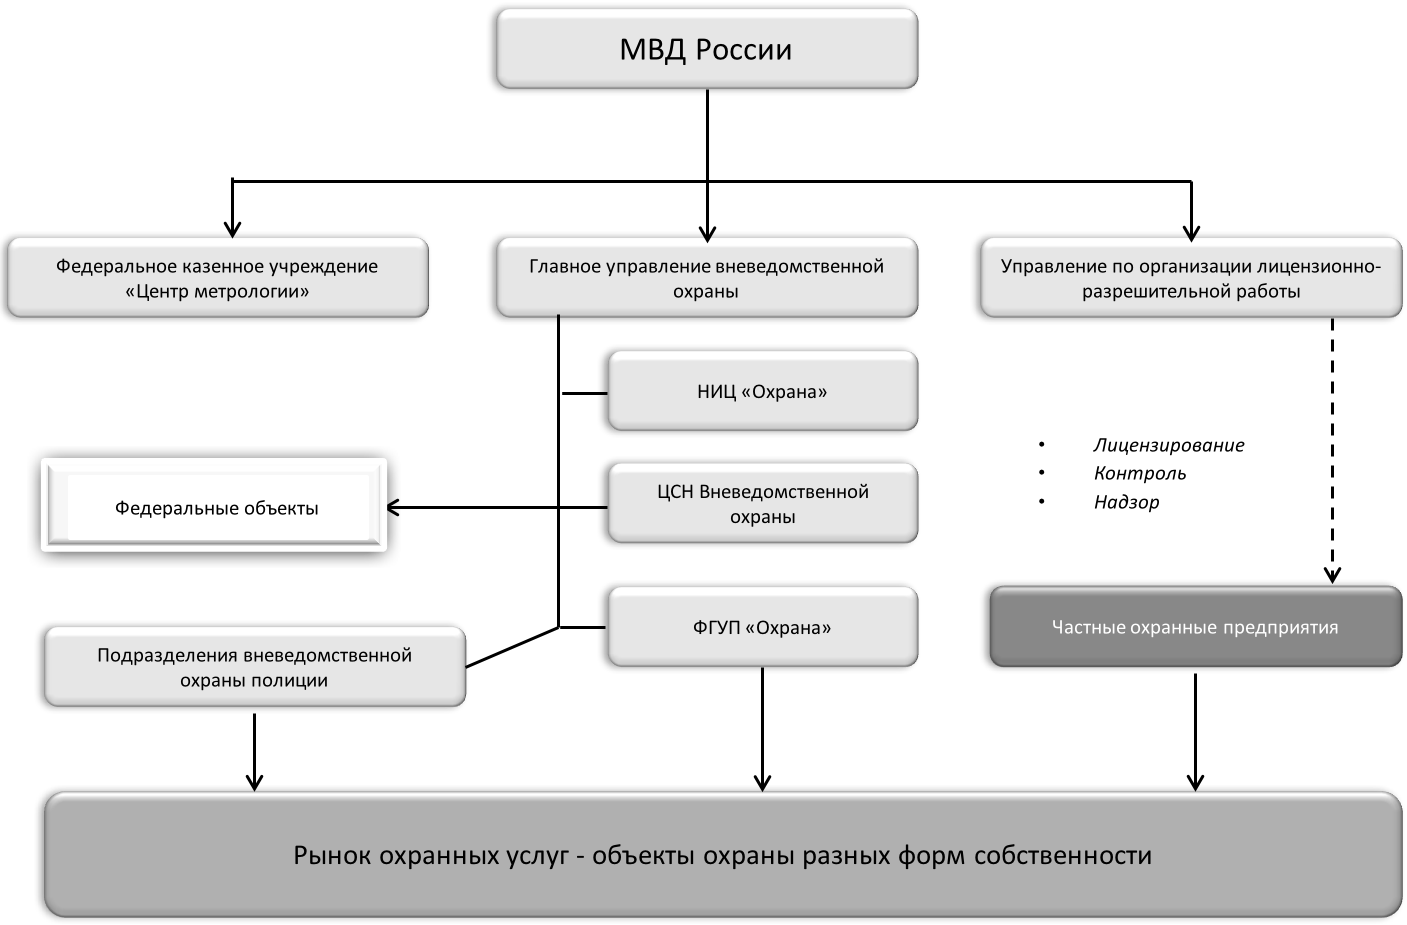
\includegraphics[scale=0.7]{img6}
	\caption{МВД России на рынке охранных услуг}
	\label{image6}
\end{figure}

Из приведенной выше схемы следует, что Министерство внутренних дел Российской Федерации осуществляет физическую и техническую охрану не только объектов государственной и муниципальной собственности, но иных объектов вне зависимости от формы собственности на свободном рынке охранных услуг. Эти функции выполняет Главное управление вневедомственной охраны, методологически подчиненные ему подразделения вневедомственной охраны территориальных органов полиции, а также находящееся в ведении МВД России ФГУП «Охрана» и его дочерние предприятия на всей территории страны. Все это вместе составляет более 60\% общего рынка охранных услуг. Характерно, что в состав главка также входит Научно-исследовательский центр «Охрана», который разрабатывает средства инженерно-технической безопасности, применяемые в совместной деятельности подразделениями вневедомственной охраны полиции, а также всеми филиалами ФГУП «Охрана». В системе МВД России также действует ФКУ «Центр метрологии», который разрабатывает, внедряет и контролирует единый порядок технического обеспечения деятельности министерства, включая средства охранной и противопожарной сигнализации. Более того, в структуру МВД России входит Управление по организации лицензионно-разрешительной работы и профильные подразделения, входящие в состав территориальных органов полиции. Они осуществляют лицензирование частной детективной и охранной деятельности, прием государственных квалификационных экзаменов, контроль соблюдения частными охранными предприятиями требований действующего законодательства, а также надзор за хранением и применением служебного ручного огнестрельного оружия и патронов к нему.

Таким образом, на рынке охранных услуг в нашей стране исторически сложилась диспропорция, благодаря которой МВД России не только устанавливает обязательные для исполнения всеми участниками рынка стандарты, не только лицензирует деятельность частных охранных предприятий и осуществляет надзор за ними, но и само участвует в конкуренции за право предоставления охранных услуг потребителям. Такое положение связано с тем, что до 1991 г. в России охранные услуги осуществлялись только представителями государства. С момента возникновения института частной собственности, а также собственной индустрии безопасности, сфера оказания охранных услуг государством несколько сократилась, но по-прежнему доминирует на рынке.

Общие подходы к организации физической охраны объектов в целом идентичны, однако в деятельности подразделений вневедомственной охраны полиции и связанных с ними филиалами ФГУП «Охрана» существует определенная специфика (см. рисунок \ref{image7}).

\begin{figure}[h]
	\centering
	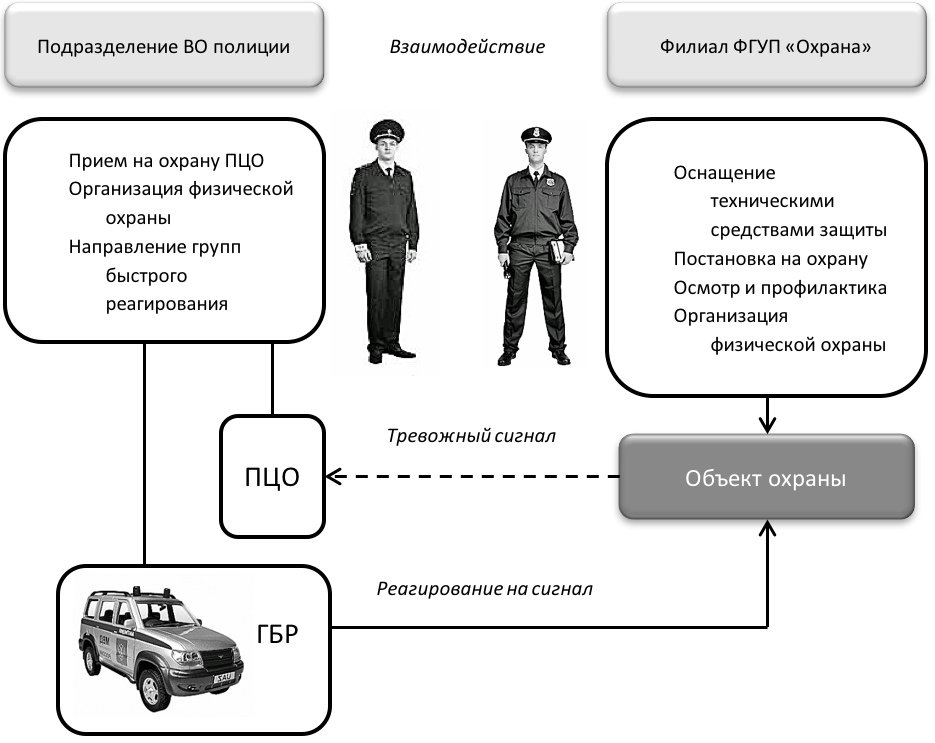
\includegraphics[scale=0.7]{img7}
	\caption{Взаимодействие вневедомственной охраны полиции и ФГУП «Охрана»}
	\label{image7}
\end{figure}

Эта специфика обусловлена тем, что ранее система вневедомственной охраны МВД составляла единое целое, в последующем из нее была выведена часть персонала совместно с профильными функциями, которые послужили основой для создания ФГУП «Охрана» и его филиалов на территории Российской Федерации. Данное предприятие осуществляет установку на охраняемых объектах систем сигнализации, выводит их на контроль в ПЦО (пульт централизованной охраны) вневедомственной охраны полиции, а также осуществляет платное техническое обслуживание в процессе эксплуатации. Полиция, в свою очередь, обеспечивает круглосуточное функционирование ПЦО и оперативное реагирование на тревожные сигналы с объектов охраны путем направления групп быстрого реагирования (ГБР). Традиционно вневедомственная охрана полиции осуществляет физическую охрану объектов путем выставления постов, вооруженных боевым оружием и специальными средствами. После создания ФГУП «Охрана» его подразделения также стали оказывать услуги предоставления физической охраны, которая может быть вооружена служебным оружием и специальными средствами или не иметь такового.

\subsection{Порядок осуществления государственной охраны}

\definition{Государственная охрана}{функция федеральных органов исполнительной власти в сфере обеспечения безопасности объектов государственной охраны, осуществляемая на основе совокупности правовых, организационных, охранных, режимных, технических и иных мер.}

Объектами государственной охраны являются лица, к которым относятся высшее должностное лицо страны - Президент РФ, лица, занимающие государственные должности Российской Федерации, федеральные государственные служащие, главы иностранных государств и правительств и иные лица иностранных государств во время пребывания на территории Российской Федерации. Охраняемыми объектами являются здания, сооружения, в которых расположены федеральные органы государственной власти, прилегающие к ним территории и акватории.

Государственная охрана осуществляется специальными федеральными органами государственной охраны, которые состоят из Федеральной службы охраны Российской Федерации и входящей в ее состав Службы безопасности Президента РФ. Федеральная служба охраны осуществляет охрану: 

\begin{itemize}
	\item Президента Российской Федерации (пожизненно);
	\item Председателя Правительства Российской Федерации (здесь и далее - на период исполнения должностных полномочий); 
	\item Председателя Совета Федерации Федерального Собрания; 
	\item Председателя Государственной Думы Федерального Собрания; 
	\item Председателя Конституционного Суда Российской Федерации; 
	\item Председателя Верховного Суда Российской Федерации; 
	\item Генерального прокурора Российской Федерации;
	\item Председателя Следственного комитета Российской Федерации.
\end{itemize}

При необходимости по решению Президента России государственная охрана может быть предоставлена другим лицам - депутатам, государственным служащим. В соответствии с международными договорами обеспечивается безопасность глав иностранных государств и правительств, членов их семей в период пребывания на территории Российской Федерации.	Служба безопасности Президента РФ также осуществляет охрану членов его семьи, проживающих с ним или его сопровождающих лиц, в течение срока полномочий Президента, а по его истечении государственная охрана предоставляется Президенту РФ  пожизненно.

Задачами, стоящими перед федеральными органами государственной охраны, являются выявление угрозы жизненно важным интересам охраняемых лиц и объектов государственной охраны, осуществление мер по предотвращению этих угроз, обеспечение безопасности объектов государственной охраны в местах постоянного и временного пребывания и на трассах проезда, обеспечение организации и функционирования президентской связи, участие в борьбе с терроризмом, выявление, предупреждение и пресечение преступлений на охраняемых объектах. Государственная охрана осуществляется путем реализации следующих мер:

\begin{itemize}
	\item Предоставление объектам государственной охраны персональной охраны, специальной связи и транспортного обслуживания;
	\item Проведение охранных мероприятий и поддержания общественного порядка в местах постоянного и временного пребывания объектов государственной охраны;
	\item Поддержание порядка и пропускного режима на охраняемых объектах.
\end{itemize}

Для осуществления этих мер федеральные органы государственной охраны вправе:

\begin{itemize}
	\item Привлекать силы и средства обеспечения безопасности (органы внутренних дел, внутренние войска и др.), необходимые для участия в подготовке и проведении охранных мероприятий; 
	\item Проверять у граждан и должностных лиц документы, удостоверяющие их личность, производить при въезде (выезде) на охраняемые объекты личный досмотр граждан, принадлежащих им вещей, транспортных средств; 
	\item Задерживать и доставлять в органы внутренних дел лиц, совершивших правонарушения в местах постоянного или временного пребывания объектов государственной охраны; 
	\item Вносить в федеральные органы государственной власти, органы государственной власти субъектов Российской Федерации, органы местного самоуправления, организации независимо от форм собственности обязательные для исполнения представления об устранении причин и условий, порождающих угрозу безопасности объектов государственной охраны и охраняемых объектов; 
	\item Использовать транспортные средства предприятий, а в неотложных случаях - и граждан для предотвращения преступления, преследования и задержания лиц, совершивших преступление или подозреваемых в его совершении; 
	\item Беспрепятственно входить в жилые и иные принадлежащие гражданам помещения, земельные участки при пресечении преступлений, а также при преследовании лиц, подозреваемых в их совершении; ведомственную принадлежность их подразделений, помещений и транспортных средств; обмениваться со специальными службами и организациями иностранных государств служебной информацией и договариваться об условиях и порядке обеспечения личной безопасности объектов государственной охраны при их выезде за пределы Российской Федерации.
\end{itemize}

С реализацией данных полномочий ФСО руководители предприятий и организаций могут столкнуться при посещении охраняемыми лицами своих объектов. 

Сотрудниками федеральных органов государственной охраны являются военнослужащими. Они проходят службу в соответствии с законодательством, с учетом особенностей деятельности органов государственной охраны. Законные требования сотрудников ФСО обязательны для исполнения всеми гражданами и должностными лицами. Никто, кроме прямых и непосредственных начальников, не вправе вмешиваться в их служебную деятельность. При исполнении своих служебных обязанностей к сотруднику федеральных органов государственной охраны не допускается применение административных взысканий, привод, административное задержание, его личный досмотр и досмотр его вещей и транспортных средств без представителя соответствующего органа государственной охраны или без решения суда. В своей служебной деятельности сотрудники федеральных органов государственной охраны не вправе руководствоваться решениями политических партий, им запрещается совмещение службы в федеральных органах государственной охраны с другой оплачиваемой работой, коммерческой деятельностью, оказывать содействие физическим и юридическим лицам в осуществлении такой деятельности (см. рисунок \ref{image8})\footnote{Информационный портал Яндекс: http://terminovo.com/catalog/article\_info.php?article\_id=139 (дата обращения: 16.03.2015)}.

\begin{figure}[h]
	\centering
	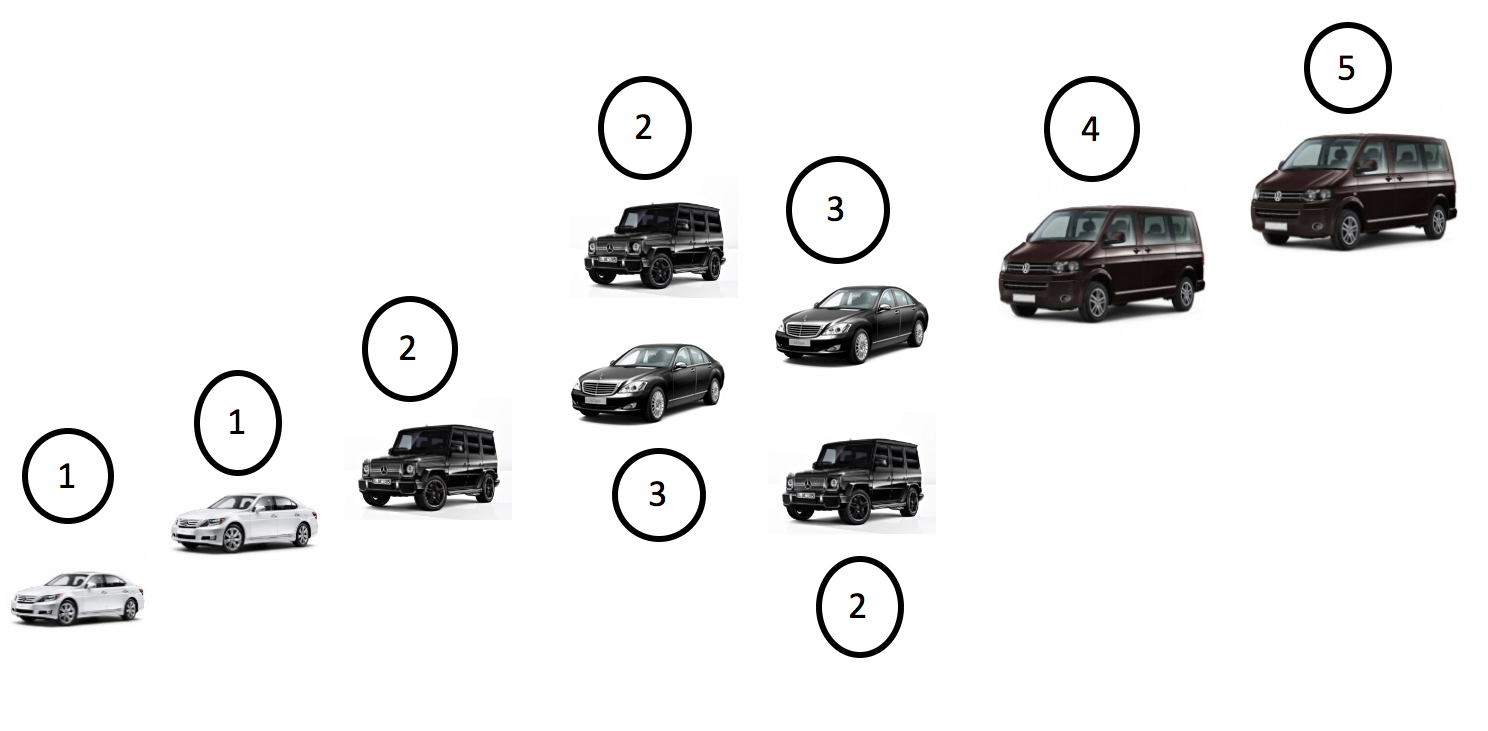
\includegraphics[scale=0.6]{img8}
	\caption{Часть кортежа президента Украины: 1 – автомобили ГАИ, 2 – автомобили охраны, 3 – автомобили президента, 4 – автомобиль спецсвязи, 5 – автомобиль охраны с тяжелым вооружением}
	\label{image8}
\end{figure}

Надзор за исполнением законов федеральными органами государственной охраны осуществляет прокуратура. Полномочия прокурора при осуществлении надзора определяются действующим законодательством. В предмет надзора не входят организация, тактика, методы и средства осуществления деятельности федеральных органов государственной охраны. 	Судебный контроль осуществляется в ходе рассмотрения судом жалоб на незаконные действия и решения органов государственный охраны, нарушающие их права или причинившие им убытки. 	Государственный контроль за деятельностью федеральных органов государственной охраны осуществляют Президент и Правительство Российской Федерации. Члены Совета Федерации и депутаты Государственной Думы вправе получать сведения о деятельности федеральных органов государственной охраны при осуществлении ими депутатской деятельности.

Во время зарубежных поездок президента любой страны сопровождает значительный персонал, включая персонал личной охраны. К примеру, при выездах президента США Дж. Буша – старшего в другие страны его сопровождали\footnote{Информационный портал Яндекс: http://xage.ru/samyie-populyarnyie-novosti-iynya/ (дата обращения: 16.03.2015)}: 250 агентов Секретной службы, 150 советников по национальной безопасности, 200 представителей других департаментов администрации, 50 политических помощников из службы Белого дома, 15 кинологов со служебными собаками, 1 персональный повар и его команда из 4-х помощников.\\

\begin{tcolorbox}[colback=blue!40!red!1!,colframe=blue!40!red,enforce breakable,% use only breakable in the real world!
	pad at break=1mm, title=Вопросы и задания для самоконтроля]
	\begin{itemize}
		\item[{\color{blue!55!red}\Huge { $ ? $}} ]  Может ли выступить коммерческий банк, согласно российскому законодательству, учредителем частного охранного предприятия?
		\item[{\color{blue!55!red}\Huge {  $ ? $}} ] Расскажите о нормативно-правовом статусе частных военно-охранных компаний в Российской Федерации.
		\item[{\color{blue!55!red}\Huge {  $ ? $}} ] Сообщите о предприятиях, учреждениях и организациях, наделенных правом создавать вооруженную ведомственную охрану.
		\item[{\color{blue!55!red}\Huge {  $ ? $}} ] Расскажите о структуре услуг, предоставляемых вневедомственной охраной полиции и подведомственными ей учреждениями.
		\item[{\color{blue!55!red}\Huge {  $ ? $}} ] Приведите примеры правомерного влияния государственной охраны на деятельность предприятий и организаций.
	\end{itemize}		
\end{tcolorbox}

\section{Инкассация денежных средств}

\begin{tcolorbox}[colback=blue!40!red!10!,colframe=blue!40!red]
В результате изучения главы студент должен \textbf{знать} основные функции обеспечения сохранности наличных денежных средств и иных материальных ценностей в процессе их инкассации; \textbf{уметь} определять правовые особенности деятельности в  области инкассации организаций с особыми уставными задачами, а также небанковских кредитных организаций, имеющих лицензию на осуществление инкассации; \textbf{владеть} правилами осуществления инкассации, особенностями подбора и расстановки кадров, современными тенденциями совершенствования деятельности инкассации.
\end{tcolorbox}

\subsection{Порядок создания и функционирования организаций с особыми уставными задачами}

Предприятия и организации, на которые законодательством Российской Федерации возложены функции, связанные с использованием и применением служебного оружия, являются юридическими лицами с особыми уставными задачами. Указанные юридические лица  имеют право в соответствии с нормативными правовыми актами Правительства Российской Федерации приобретать гражданское и служебное оружие у юридических лиц-поставщиков после получения соответствующей лицензии в органах внутренних дел. Виды, типы, модели и количество гражданского и служебного оружия, которое имеют право приобретать юридические лица с особыми уставными задачами, устанавливаются Правительством Российской Федерации.

Ряд организаций с особыми уставными задачами имеют право получать во временное пользование в органах внутренних дел отдельные типы и модели боевого ручного стрелкового оружия:

\begin{itemize}
	\item Центральный банк Российской Федерации;
	\item Российское объединение инкассации при Банке России;
	\item ОАО «Сбербанк России»;
	\item Главный центр специальной связи; 
	\item Фельдъегерская служба МИД России; 
	\item Иные юридические лица с особыми уставными задачами, за исключением частных охранных предприятий и служб безопасности организаций, которые имеют право получать во временное пользование в органах внутренних дел для исполнения возложенных на них федеральным законом обязанностей по: 
	\begin{itemize}
		\item Охране объектов производства и хранения оружия, боеприпасов, боевой техники; 
		\item Охране особо опасных экологических производств, природы и природных ресурсов; 
		\item Охране мест изготовления и хранения денежных средств и ценностей; 
		\item Охране мест добычи, переработки и хранения драгоценных металлов и драгоценных камней; 
		\item Охране дипломатических представительств Российской Федерации в иностранных государствах, других особо важных объектов; 
		\item А также при транспортировании особо опасных грузов, оружия, боеприпасов, боевой техники, денежных средств и ценностей, дипломатической почты, корреспонденции, содержащей сведения, отнесенные к государственной тайне, и грузов, содержащих носители сведений, отнесенных к государственной тайне.
	\end{itemize}
\end{itemize}

Вопрос об использовании оружия имеет прямое отношение к деятельности любого подразделения инкассации, ведь перевозимые денежные средства и иные ценности нуждаются в надежной защите. Вместе с тем, в финансовой системе инкассация считается одной из банковских операций. Ведь инкассация - это не только перевозка денег, но и пересчет наличных купюр, их упаковка, выбраковка, документальное оформление факта передачи денежных средств от клиента. В процесс инкассации добавляются еще и многочисленные чисто технические инструменты. Поэтому финансовыми операциями в процессе инкассации занимается, как правило, банковский работник (или финансовый работник организации-заказчика), а перевозкой и охраной – представители организаций  с особыми уставными задачами.

Банк России самостоятельно осуществляет доставку денежного подкрепления в регионы страны, для чего обладает собственным структурным подразделением, оснащенным специальными средствами транспорта и боевым огнестрельным оружием. В систему Банка России также входит Российское объединение инкассации (Росинкассо), оказывающее профильные услуги клиентам внутри регионов. Это объединение является одновременно организацией с особыми уставными задачами (вооружено боевым стрелковым оружием) и лицензированной службой инкассации. Аналогичными функциями и полномочиями обладает служба инкассации ОАО «Сбербанк России» - крупнейшего финансово-кредитного учреждения страны (см. рисунок \ref{image9}).

\begin{figure}[h]
	\centering
	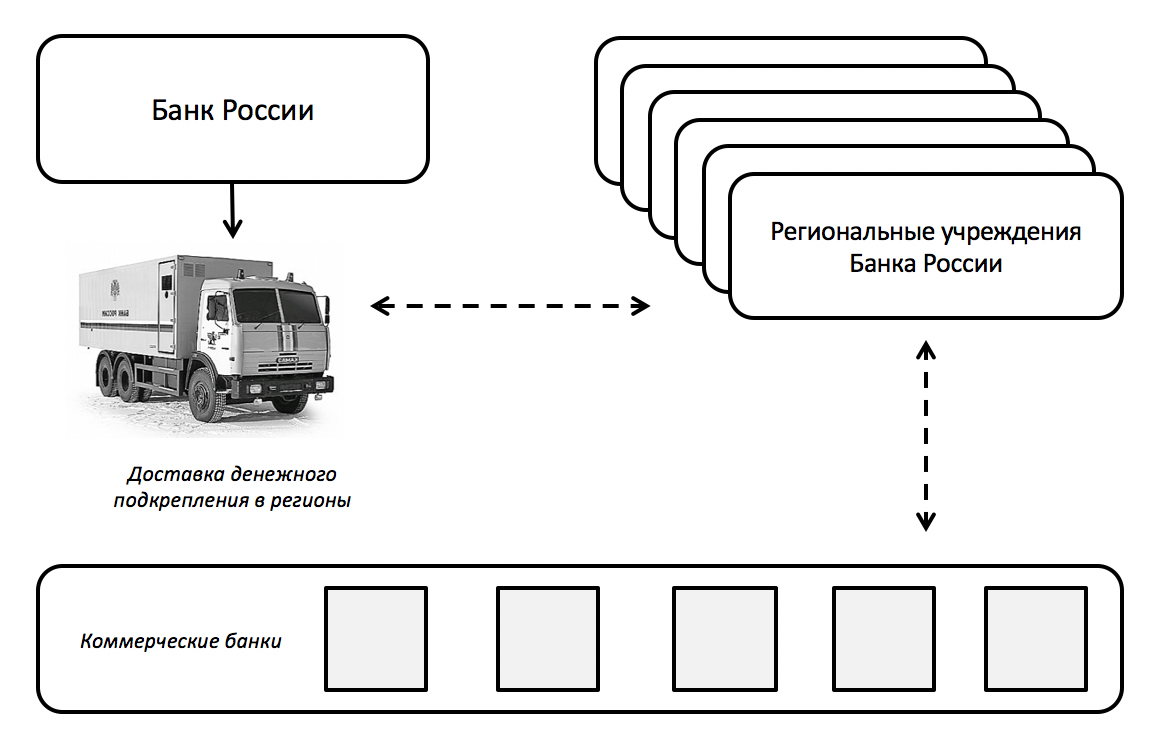
\includegraphics[scale=0.7]{img9}
	\caption{Схема обращения денежной наличности на территории РФ}
	\label{image9}
\end{figure}.

Другие банки создают собственные службы инкассации или пользуются услугами профессиональных операторов данного рынка: Росинкассо, службы инкассации ОАО «Сбербанк России» или самостоятельных служб инкассации, имеющих ограниченную лицензию на совершение банковских операций. Такие службы, как правило, создают совместные предприятия с частными охранными структурами, имеющими лицензию на охранную деятельность и обладающими служебным огнестрельным оружием на законных основаниях. В ряде случаев сотрудники таких совместных предприятий используют бронированные автомобили, единую форменную одежду. В состав их бригад входят: инкассатор, водитель-охранник и охранник.

Профессиональные службы инкассации используются коммерческими банками для доставки денежной наличности предприятиям и организациям для обеспечения товарно-денежного оборота в розничной торговле, общественном питании и иных сферах работ, предусматривающих оборот наличных денежных средств. Излишки денежной наличности (согласно разрешенному кассовому остатку) регулярно изымаются из названных выше учреждений и доставляются в банк для зачисления на счет организации. В ряде городов, в которых действуют крупные торговые центры и гипермаркеты, работа служб инкассации осуществляется на круглосуточной основе (см. рисунок \ref{image10}). Деятельность бригад инкассации координируется соответствующими центрами мониторинга и подчиняется в большинстве случаев законам логистики при формировании маршрутов, включающих в себя временные позиции операций по инкассации, согласованные с клиентами. Службы инкассации в своей работе используют бронированные автомобиля различных классов, средства радиосвязи со своими центрами мониторинга. Автомобили инкассации в большинстве случаев оснащены средствами пассивного мониторинга их передвижения по маршруту, обозначенному в путевом листе. Спутниковая связь с центром также позволяет бригадам инкассаторов поддерживать дополнительный канал связи с центром мониторинга через спутник. Инкассаторы также оснащены средствами личной связи. 

\begin{figure}[h]
	\centering
	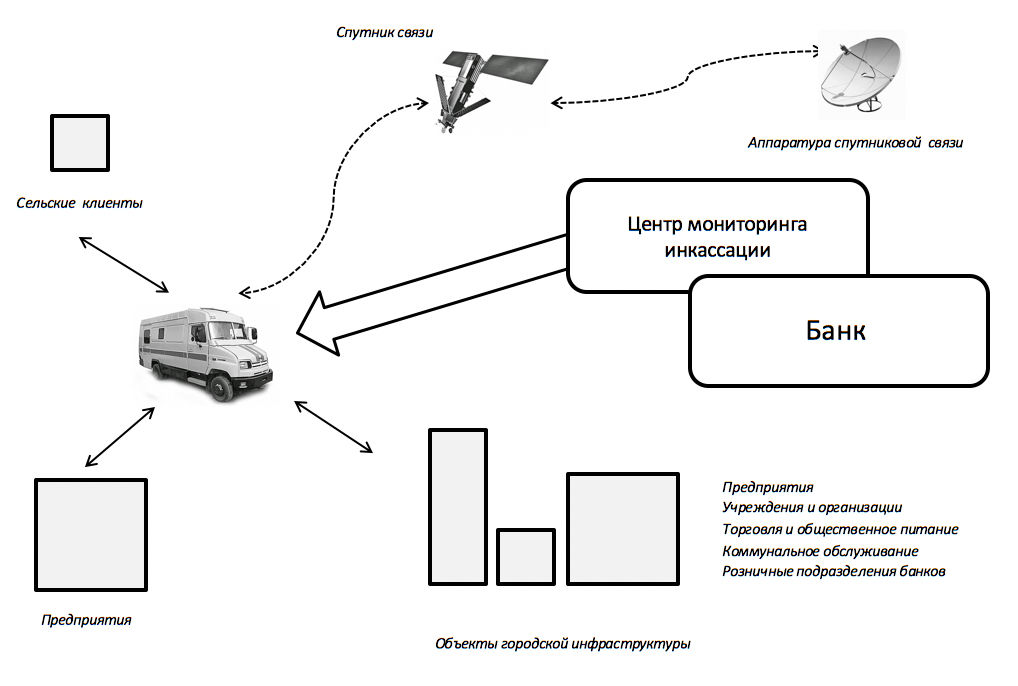
\includegraphics[scale=0.9]{img10}
	\caption{Схема обращения наличных денег в системе банк-клиент}
	\label{image10}
\end{figure}.

Существенная доля рынка инкассации принадлежит банковским службам, которые удерживают клиентов не только качеством непосредственно услуг перевозчика, но и дополнительными банковскими продуктами. В такой ситуации успех вхождения на рынок может быть гарантирован лишь привлекательным для клиентов сочетанием всей линейки банковских продуктов, что может обеспечить лишь весьма ограниченная группа банков. На современном рынке сохранилась тенденция на консолидацию, в соответствии с которой все большее число банков отказывается от содержания собственной службы инкассации в пользу передачи данной функции на аутсорсинг. Это продиктовано, прежде всего, низкой рентабельностью данного направления бизнеса особенно для небольших банков с высокими удельными издержками. С другой стороны, нарастание рисков внутри банковской системы стало способствовать желанию крупных торговых сетей, являющихся наиболее значимыми клиентами инкассаторов, диверсифицировать риски. Следствием чего распространённой ситуацией стало одновременное обслуживание одной и той же торговой сети сразу несколькими перевозчиками. В результате тенденция концентрации рынка дополнилась тенденцией выравнивания долей рынка инкассаторских услуг среди крупнейших его участников.

Тенденции на мировом рынке инкассации связаны со следующими  определяющими факторами: сокращением числа профессиональных участников рынка; повышением профессионализма остающихся операторов услуг инкассации и поэтапным переходом к снижению традиционных профессиональных рисков. Такая тенденция с опережением по отношению к России на 10-12 лет наблюдается в США, Японии и развитых странах ЕС. Многие службы инкассации зарубежных стран перешли на перевозку наличных денежных средств в специальных контейнерах, оборудованных устройствами в виде химических или дымовых ловушек и маркеров. В настоящее время такие устройства могут срабатывать автоматически - в случае нападения они позволяют остановить преступника в силу бессмысленности его действий. Снижение рисков попадания наличных денежных средств позволяет сократить использование в службе инкассации огнестрельного оружия и как следствие, существенно снизить риски убийств инкассаторов или нанесения им тяжких телесных повреждений. 

Еще одной особенностью рынка инкассации является тот факт, что Банк России является регулятором этого вида финансово-кредитных операций с одной стороны, а с другой его собственная дочерняя компания Росинкассо одновременно участвует в конкурентной борьбе на этом рынке услуг.

\subsection{Порядок создания и функционирования небанковских кредитных организаций}

Существующим законодательством определены три категории небанковских кредитных организаций: 

\begin{itemize}
	\item Расчетная небанковская кредитная организация;
	\item Платежная небанковская кредитная организация (небанковская кредитная организация, имеющая право на осуществление переводов денежных средств без открытия банковских счетов и связанных с ними иных банковских операций);
	\item Кредитно-депозитная небанковская кредитная организация.
\end{itemize}

Основные положения о порядке создания и функционирования небанковских кредитных организаций регламентируются специальным указанием Банка России о регистрации небанковских кредитных организаций, осуществляющих операции по инкассации, и особенностях лицензирования их деятельности. При этом все   организации,   создаваемые  для  осуществления инкассации (прием,  доставка  и  сдача)  денежных средств,  векселей, платежных и расчетных документов,  подлежат регистрации в Банке России в качестве небанковских кредитных организаций. В зависимости от функционального назначения такие организации могут осуществлять обслуживание юридических лиц, в том числе кредитных организаций, на межбанковском, валютном рынках и рынке ценных бумаг. НКО могут производить расчеты по пластиковым картам, инкассацию денежных средств, векселей, платежных и расчетных документов, а также кассовое обслуживание юридических лиц и операции по купле-продаже иностранной валюты в безналичной форме. 

Главное различие между НКО и коммерческим банком состоит в том, что НКО не имеет права размещать денежные средства от своего имени и заниматься инвестиционной деятельностью. Деньги, не ушедшие со счетов небанковской кредитной организации, не могут принести ей дополнительных доходов. Следовательно, отсутствуют кредитные риски и риск потери ликвидности и платежеспособности из-за непрофессионального управления средствами клиентов и вложения их в высоко рискованные виды активов. Таким образом, из деятельности небанковской кредитной организации исключаются основные риски, связанные с возможным неисполнением долговых обязательств, понижением стоимости ценных бумаг, изменением курса иностранной валюты. Инкассация денежных средств,  векселей,  платежных и расчетных документов, в соответствии с предписанием ЦБ РФ, должна  быть  обеспечена  надежной  охраной.  

Охрана  может осуществляться организацией,  специализирующейся   на   предоставлении такого рода услуг, на основании   соответствующего   договора  с небанковской кредитной организацией,  либо осуществляется  собственной службой безопасности небанковской кредитной организации. В случае если охрана будет осуществляться собственной службой безопасности, небанковская  кредитная  организация после регистрации в Банке России должна согласовать устав службы  безопасности  в  органах внутренних дел  по месту своего нахождения. Для получения лицензии на осуществление операции по  инкассации    небанковская кредитная организация должна  представить  в  территориальное  учреждение  Банка России нотариально удостоверенные копии следующих документов:  

\begin{itemize}
	\item Согласованного  с органами внутренних дел устава службы безопасности;  
	\item Разрешения органа внутренних дел  на  хранение  и   использование   служебного   оружия;
	\item Документов, подтверждающих   право   собственности   или   аренды   на  автомобили.
\end{itemize}

Если  охрана  инкассации  будет  осуществляться  организацией, специализирующейся на охранной  деятельности,  небанковская  кредитная организация для   получения  лицензии  на  осуществление  операции  по инкассации должна  представить  в  территориальное  учреждение   Банка России также нотариально   удостоверенные   копии   следующих документов  организации, специализирующейся на   охранной   деятельности:    

\begin{itemize}
	\item Уставных документов;    
	\item Лицензии    на    охранную деятельность; 
	\item Разрешения  органа  внутренних   дел   на   хранение   и использование служебного   оружия;   
	\item Договора   на   охрану  с  данной организацией и документов организации инкассации, подтверждающих право собственности или аренды на автомобили.
\end{itemize}

Для организации инкассации денежных средств в организации необходимо создание инфраструктуры направления, а именно: 

\begin{itemize}
	\item Дежурного отделения с необходимым персоналом и оборудованием; 
	\item Экипажей машин инкассации – основного и резервного; 
	\item Группы быстрого реагирования. 
\end{itemize}

Наличие дежурного отделения, как и группы быстрого реагирования, для многих охранных предприятий вопрос уже решенный, так как одним из самых распространенных видов услуг охраны является пультовое централизованное наблюдение. Вместе с этим при организации инкассации охранному предприятию необходимо пересматривать концепцию полевого расположения групп быстрого реагирования, а также технически «перевооружать» свой пункт централизованного наблюдения (мониторинга). 

Контроль инкассации требует наличия дополнительного рабочего места в пункте централизованного наблюдения, на который будет сводиться оперативная связь с инкассаторскими экипажами, а также выводиться данные о местонахождении инкассаторских автомобилей. Экипаж инкассаторского автомобиля, как правило, состоит из трех человек, а именно: 

\begin{itemize}
	\item Водитель. Осуществляет оперативную связь с пунктом централизованного наблюдения и ведет бронеавтомобиль по установленному маршруту; 
	\item Инкассатор. Осуществляет непосредственный контакт с клиентами, выемку денежных средств из банкоматов и т.д.; 
	\item Охранник. Остается в автомобиле и осуществляет охрану уже имеющихся денежных средств в бронеавтомобиле, а также отслеживает оперативную обстановку в момент инкассации. При инкассации большого количества денег в состав экипажа может входить два охранника, один из которых остается в фургоне, а второй осуществляет прикрытие инкассатора. 
\end{itemize}

Начинающий инкассатор должен пройти месячный теоретический курс обучения, а затем сдать зачет по теоретической части и физической подготовке. В течение всего месяца новобранцы изучают теорию и одновременно проходят практическое обучение на маршрутах инкассации. На теорию отведено 46 часов, а на практику – 108 часов. Теоретические занятия производятся по следующим предметам: специальная подготовка, физическая подготовка, техническая подготовка, основы законодательства и права, психологическая подготовка и медицинская подготовка. Обучение организуется с учетом того, если у инкассатора опыт аналогичной работы. После окончания испытательного срока инкассаторы подвергаются контрольным экзаменам, а затем принимается окончательное решение по нахождению в должности. Как и на любой работе, у сотрудников инкассаторской службы возможен карьерный рост. \\

\textit{Должностные обязанности инкассатора}\\

Круг работы инкассаторов достаточно широкий. Однако, чаще всего обязанности инкассатора состоят в подготовке к подготовке к началу работы, получению в соответствии с установленным порядком в кассе компании денежных средств или ценных бумаг и доставке их в учреждения банка по месту нахождения расчетного или же текущего счета, доставке в организацию из банка денежной наличности. Все это выполняется в соответствии с регламентом.\\

\textit{Оружие инкассатора}\\

Для каждого инкассатора выделяется служебное оружие. Однако перед этим инкассатору необходимо сдать экзамен в районном отделении лицензировано-разрешительной системы МВД. Данный экзамен имеет две части. Первая – письменная, на которой инкассатор должен ответить на письменные вопросы о служебном оружии: тактико-технические характеристики, правила ношения и применения оружия и спецсредств (дубинки, наручники, слезоточивый газ), а также проверка знаний определенных статей Уголовного кодекса РФ. Вторая часть экзамена – стрельба. Чаще всего из пистолета Марголина, ИЖ. Затем выдает лицензия на оружие, и инкассатор имеет право заниматься транспортировкой и охраной денежных средств и ценностей. Инкассатор не имеет права использовать табельное оружие в местах массового скопления людей, против несовершеннолетних и женщин (если конечно эти лица не совершают вооруженного нападения на инкассацию) и граждан с детьми. Применять оружие инкассаторы могут только в трех случаях:

\begin{itemize}
	\item Защита перевозимых денег и других материальных ценностей;
	\item Защита собственной жизни инкассатора в случае нападение преступника;
	\item Задержание преступника после нападения.
\end{itemize}

О каждом факте использования оружия инкассатор обязан доложить в полицию и находиться на месте происшествия до прибытия правоохранительных органов, если конечно отсутствует вероятность повторного нападения.\\

\textit{Инкассаторская машина}\\

После прохождения обязательного ежедневного медицинского осмотра, инструктажа и получения оружия инкассаторы садятся в бронированный автомобиль и отправляются на маршрут. Маршруты движения автомобиля предварительно согласовываются с управлением внутренних дел, а непосредственно перед выездом транспорта о его маршруте становится известно в территориальном отделении полиции. Инкассаторские автомобили могут быть разными. Во время перевозки денег инкассаторам и охранникам категорически запрещается делать остановки, не связанные с выполнением прямых служебных обязанностей, разговаривать по мобильному телефону, беседовать с посторонними лицами, открывать окна. Инкассаторы должны внимательно отслеживать обстановку вокруг автомобиля, выявлять подозрительных лиц, следующие за ними продолжительное время автомобили и докладывать в центр мониторинга.\\

\begin{tcolorbox}[colback=blue!55!red!5!,colframe=blue!55!red,enforce breakable,% use only breakable in the real world!
	pad at break=1mm, title=Кейс 34. Опасные типовые нарушения в инкассации]
	
	Меры безопасности в инкассации выработаны на основе предыдущего отечественного и зарубежного опыта, фактов утраты (насильственного захвата) денежных средств, а также гибели сотрудников инкассации при исполнении своих служебных обязанностей. По этим причинам работа инкассаторов детально регламентирована, и каждый ее элемент несет серьезную смысловую нагрузку. К примеру, как показывает опыт гласного и негласного контроля за работой бригад инкассации, люди привыкают к любой, даже весьма опасной работе. Достаточно часто инкассаторы не проверяют техническую исправность и готовность служебного автотранспорта, работоспособность средств радиосвязи, пригодность оружия к применению в штатной ситуации. В ряде случаев водитель-инкассатор, вместо того, чтобы запереть автомобиль изнутри и контролировать окружающую обстановку, оставляет свою дверь открытой, кладет на свободное сидение оружие и даже курит. При большом объеме инкассируемой в одной точке наличности инкассаторы стараются перенести как можно больше сумок за один раз. В результате у каждого из них обе руки заняты поклажей. 
	
	\begin{itemize}
		\item[{\color{blue!55!red}\Huge {  $ ? $}} \quad]   Предположите возможные последствия описанных нарушений.
	\end{itemize}	
	
\end{tcolorbox}

\textit{Инкассаторская сумка}\\

Денежные средства или другие ценности перевозятся в специализированных инкассаторских сумках. Инкассаторская сумка разработана специально для транспортировки либо хранения крупных денежных сумм и ценных бумаг с учетом всевозможных рисков при перевозке. 

Во время маршрута инкассаторская сумка с деньгами и ценностями находится под ответственностью старшего бригады инкассаторов в сейфе, металлическом ящике или мешке, а по окончанию заезда старший бригады инкассаторов отдает принятые ценности в кассу банка. Стандартные инкассаторские сумки изготавливают из прочного материала, который исключает возможность возгорания или промокания. Благодаря этому, ни одна купюра или ценная бумага не может быть испорчена. 	На инкассаторской сумке имеется специальная планка с замком. Замок оборудован приспособлением, которое используется для пломбирования. Опломбирование может производиться при помощи банковского свинцовой пломбы и трехжильного шпагата. Помимо этого, применяются одноразовые номерные пломбы. Их изготавливают из пластика или металла. Это очень надежный механизм, который исключает повторное применение после вскрытия, так как вскрыть сумку с одноразовой пломбой без её повреждения невозможно. Подделка такой одноразовой пломбы тоже практически невозможна. Указанные приспособления надежно защищают деньги от несанкционированных действий персонала, однако они не могут считаться защитой от преступников, захвативших сумки с ценным грузом.\\

\begin{tcolorbox}[colback=blue!40!red!1!,colframe=blue!40!red,enforce breakable,% use only breakable in the real world!
	pad at break=1mm, title=Вопросы и задания для самоконтроля]
	\begin{itemize}
		\item[{\color{blue!55!red}\Huge { $ ? $}} ]  Дайте определение понятия «инкассация» денежных средств.
		\item[{\color{blue!55!red}\Huge {  $ ? $}} ] Приведите примеры и сведения об организациях с особыми уставными задачами.
		\item[{\color{blue!55!red}\Huge {  $ ? $}} ] Дайте определение понятия «небанковская кредитная организация».
		\item[{\color{blue!55!red}\Huge {  $ ? $}} ] Расскажите о требованиях Банка России к подразделениям инкассации коммерческих банков.
		\item[{\color{blue!55!red}\Huge {  $ ? $}} ] 
		Расскажите о тенденциях развития и инновациях в сфере инкассации.
	\end{itemize}		
\end{tcolorbox}

\section{Взаимодействие частных и государственных институтов}

\begin{tcolorbox}[colback=blue!40!red!10!,colframe=blue!40!red]
В результате изучения главы студент должен \textbf{знать} контрольные функции государства в области лицензирования физических и юридических лиц, осуществляющих охранную деятельность, контроля их служебной деятельности; \textbf{уметь} вычленять  вопросы взаимодействия частных и государственных институтов в сфере обеспечения физической охраны объектов, в области обеспечения общественной безопасности и правопорядка, а также при расследовании инцидентов в сфере обеспечения физической безопасности на базе правовых и организационных основ; \textbf{владеть} правовыми основами взаимодействия субъектов предпринимательской деятельности с государственными институтами в области обеспечения физической безопасности.
\end{tcolorbox}

\subsection{Лицензирование частной охранной деятельности}

\definition{Частная охранная деятельность}{негосударственная правоохранительная деятельность, осуществляемая специализированными негосударственными организациями на основе лицензии, выдаваемой уполномоченным федеральным органом исполнительной власти в установленном законом порядке.}

В главе 3 настоящего раздела было показано, что частное охранное предприятие признается субъектом гражданского права после его государственной регистрации. Государственная же регистрация указанного вида предприятий возможна только при наличии лицензии на занятие частной охранной деятельностью. Иными словами, лицензия на занятие частной охранной и детективной деятельностью, выдаваемая частному охранному или детективному предприятию, есть основание для его государственной регистрации в качестве юридического лица — субъекта гражданского права.

Одной из правовых целей наделения охранно-детективных субъектов специальной правоспособностью является предоставление им только тех гражданских прав и возложение на них только таких обязанностей, которые соответствуют целям и предмету деятельности. При этом необходимо отметить, что частная охранная деятельность лицензируется в особом порядке. 	Предоставление лицензий на осуществление частной охранной деятельности производится органами внутренних дел. Лицензия предоставляется сроком на пять лет и действует на всей территории Российской Федерации. В лицензии указывается (указываются) вид (виды) охранных услуг, которые может оказывать лицензиат. Решение о \textbf{предоставлении либо об отказе в предоставлении лицензии} принимается в срок \textbf{не более сорока пяти дней}.

Типовое положение о лицензировании частной охранной деятельности утверждается Постановлением Правительства Российской Федерации. В нем устанавливается порядок лицензирования данного вида деятельности, а также перечень лицензионных требований и условий по каждому виду охранных услуг. При этом органы внутренних дел осуществляют следующие полномочия в области лицензирования частной охранной деятельности:

\begin{itemize}
	\item Предоставление лицензии;
	\item Переоформление документов, подтверждающих наличие лицензии;
	\item Приостановление и возобновление действия лицензии в случаях, установленных настоящим Законом;
	\item Ведение реестров лицензий и предоставление сведений из них;
	\item Осуществление государственного контроля за соблюдением лицензиатами лицензионных требований и условий, а также требований законодательства Российской Федерации, регламентирующего оборот оружия и специальных средств;
	\item Обращение в суд с заявлением о приостановлении действия лицензии либо об аннулировании лицензии;
	\item Прекращение действия лицензии в случае получения письменного заявления лицензиата о прекращении им осуществления данного вида деятельности.
\end{itemize}

Для получения лицензии на осуществление частной охранной деятельности руководитель организации обязан представить в Центр лицензионно-разрешительной работы УМВД России комплект необходимых документов, включая копии учредительных документов, а также документы по каждому виду охранных услуг, предусмотренные положением о лицензировании частной охранной деятельности.

Органы внутренних дел обязаны устанавливать достоверность сведений, изложенных в представленных документах и приложениях к ним. Основанием для отказа в предоставлении лицензии является несоответствие соискателя лицензии лицензионным требованиям и условиям. В ряде случаев может потребоваться переоформление документов, подтверждающих наличие лицензии на осуществление частной охранной деятельности. Такими случаями являются:

\begin{itemize}
	\item Продление срока действия лицензии;
	\item Намерение лицензиата осуществлять новые виды охранных услуг, не указанные в предоставленной (имеющейся) лицензии;
	\item Реорганизация охранной организации;
	\item Изменение наименования охранной организации или места ее нахождения.
\end{itemize}

В первых двух случаях представляются соответствующие заявление и документы по данному виду услуг, предусмотренные Положением о лицензировании частной охранной деятельности и рассмотренные выше. 	В случае \textbf{реорганизации охранной организации либо изменения ее наименования, а также места её нахождения} данная охранная организация обязана подать в орган внутренних дел, выдавший лицензию, соответствующее \textbf{заявление в течение пятнадцати суток с момента внесения изменений в ЕГРЮЛ}. В этом случае соответствующее \textbf{переоформление документа, подтверждающего наличие лицензии}, осуществляется в срок \textbf{не более 25  дней}. На период переоформления действие лицензии не приостанавливается.

\subsection{Мониторинг частной охранной деятельности}

Контроль за деятельностью частных охранных структур в России, а именно  контроль за частной детективной и охранной деятельностью и оборотом оружия, осуществляют региональные Центры лицензионно-разрешительной работы ГУ МВД России.  В соответствии с действующим законодательством сотрудниками указанных подразделений в рамках контроля за деятельностью частных охранных организаций, образовательных учреждений, осуществляющих профессиональную подготовку охранников, проводятся проверки, в ходе которых запрашиваются соответствующие документы, а также информация, необходимая для выполнения контрольных функций. По результатам проверочных мероприятий в случае выявления нарушений сотрудником лицензионно-разрешительной работы выдаются предписания об устранении выявленных недостатков и применяются меры административного воздействия.

Человеческий фактор в проблеме охраны является определяющим, поэтому очень важна подготовка персонала. Законодательством предусмотрена трехразрядная квалификация частных охранников: 

\begin{itemize}
	\item 4-й разряд позволяет осуществлять охранную деятельность с правом использования специальных средств; 
	\item 5-й разряд предоставляет право претендовать на должности, предусматривающие использование не только специальных средств, но и гражданского оружия; 
	\item 6-й разряд выполнять работу, предусматривающую использование специальных средств, гражданского и служебного огнестрельного оружия.
\end{itemize}

При оказании охранных услуг частной охранной организацией с использованием видеонаблюдения, а также оказания охранных услуг в виде обеспечения внутриобъектового и(или) пропускного режимов персонал и посетители объекта охраны должны быть проинформированы об этом посредством размещения соответствующей информации в местах, обеспечивающих гарантированную видимость в дневное и ночное время, до входа на охраняемую территорию. Такая информация должна содержать сведения об условиях внутриобъектового контроля и пропускного режимов.

Органы полиции вправе проводить проверки соблюдения правил оборота специальных средств, оружия и патронов к нему. Условия приостановления, а также  полного лишения лицензии на частную охранную деятельность строго регламентированы. Сроки проведения \textbf{плановых выездных проверок} не могут превышать \textbf{30 дней}, а \textbf{внеплановых выездных проверок - 20 дней}. В настоящее время проверки \textbf{ЧОП со стороны органов МВД} должны проводиться \textbf{не реже 1 раза в год, а полицией на местах} - \textbf{не реже 1 раза в квартал. Плановые выездные проверки} должны проводиться \textbf{не реже одного раза в 5 лет}. Строго регламентированы и основания, по которым может быть назначена внеплановая проверка соблюдения лицензионных требований. Дополнительно ЧОП могут проверить, если раньше у предприятия уже были выявлены нарушения. Вне плана проверяющие могут придти только в случаях получения информации о нарушении ЧОПом законодательства, регламентирующего частную детективную и охранную деятельность, а также оборот оружия и специальных средств, поступившей от граждан либо от органов государственной власти и органов контроля. Регламентированы также сроки и правила реагирования органов полиции на жалобы со стороны владельцев ЧОПов: \textbf{письменное обращение} должно рассматриваться в течение \textbf{30 дней со дня его регистрации}. При этом о результатах рассмотрения обращения заявителю в письменной форме либо по его желанию в электронной форме направляется мотивированный ответ.

Служба внутреннего мониторинга МВД выделяет следующие основные претензии к полиции со стороны частных охранных предприятий:

\begin{itemize}
	\item Отсутствие нормативных оснований для проведения проверки. Это весьма редкое явление и, соответственно, нечастая претензия. Однако если уж она имеет место, то предприятия, усматривающие такое нарушение, порой предпринимают самые активные меры для признания незаконными действий сотрудника ОВД и аннулирования результатов подобных проверок – вплоть до одновременного обращения в МВД России, прокуратуру и суд.
	\item Нарушение порядка уведомления о предстоящей поверке.  Надлежит неукоснительно исполнять установление п. 8 Положения о лицензировании в части уведомления лицензиата о предстоящей плановой проверке за 3 дня.
	\item Нарушение периодичности при поведении проверки. По мнению приблизительно каждого четвертого из опрошенных экспертов, инспекторы выходят за пределы своей компетенции, осуществляя проверки слишком часто. 
	\item Проведение проверки ненадлежащими лицами. Поч­ти каждый десятый респондент высказал мнение, будто проверку осуществляли сотрудники, в чью компетенцию это не входит (например участковые), либо те, кто в одиночку не мог производить эти действия.
	\item роведение проверки в присутствии ненадлежащего лица. По мнению опрошенных, это нарушение встречается редко. В действительности, как показало изучение 535 актов проверок, примерно в каждом десятом (55 из них) в качестве присутствующих поименованы ненадлежащие лица (охранники, старшие смен и др.).
	\item Изложение в акте проверки предписаний, не соответствующих нормативным требованиям. Более того, предписания, не соответствующие нормативным требованиям (таковые зафиксированы в 243 актах) нередко адресовались тем охранным структур, чьи руководители не высказывали подобных замечаний (причем ряд предписаний можно расценить именно как выход проверяющих за рамки компетенции, предоставленной им законом).
\end{itemize}

\subsection{Совместное обеспечение безопасности и правопорядка}

Сотрудничество правоохранительных органов с частными охранниками и детективами всегда предусматривалось законами. Более того, в российском законодательстве даже указаны обстоятельства, при  которых частники обязаны оказывать всяческое содействие полиции. К примеру, по требованию полицейских предоставить записи камер видеонаблюдения, сообщить о совершенном или готовящемся преступлении. Кроме того, ЧОП нередко подключают своих сотрудников к охране общественного порядка во время массовых гуляний, а также для совместного патрулирования. Известны даже случаи, когда группы быстрого реагирования формируются из сотрудников вневедомственной охраны и сотрудников ЧОП. В этом случае, когда в группе присутствует полицейский, частные охранники получают права самостоятельно задерживать грабителей, хулиганов и воров.

Вместе с тем, в большинстве случаев сотрудничество с полицией остается делом добровольным. В настоящее время в соответствии с приказом министра внутренних дел для координации совместных действий за каждым ЧОП, которое заключило договор с МВД, закрепляется конкретный сотрудник полиции. Он находится в постоянном контакте с несколькими охранными структурами. В его обязанности входит обработка информации, поступающей от частных охранных предприятий, инструктирование и оказание помощи работникам частной охраны. В то же самое время при необходимости, он сможет вызвать их на помощь силам полиции в соответствующем районе.

Закон предоставил право негосударственой охране «оказывать содействие правоохранительным органам в решении возложенных на них задач» еще 20 лет назад. Так, охранники могут задерживать и передавать в полицию граждан, совершивших правонарушения и преступления. Однако они не имеют права самостоятельно проверять документы у задержанных и досматривать их. Оружие сотрудники охранных структур могут использовать только для самообороны. Если охранник превысил свои полномочия, применил насилие или угрожал его применить, ему грозит не только административное, но и уголовное наказание. Если при этом действия охранника привели к тяжким последствиям, он может получить до семи лет лишения свободы. 

По оценке экспертов, в охранном сообществе России есть как профессионалы экстра-класса, так и ненадежные компании, выживающие за счет дешевизны услуг. Некоторые из них являются больше частными армиями, чем открытыми компаниями. Обеспечение корпоративных интересов клиентов для них важнее выполнения законов. Такие компании меньше связаны страхом потери лицензии или реализации репутационных рисков, поэтому не все они в равной степени стремятся к ежедневному взаимодействию с органами внутренних дел. В тоже самое время ЧОПы в России пока не могут чувствовать себя полноправными партнерами государства, и государство не демонстрирует готовности к смене ситуации по западногерманскому образцу. Контроль со стороны государства остается основной темой для организации взаимодействия.  

Вместе с тем необходимо учитывать, что взаимодействие полиции и частных охранных предприятий не является единственным направлением во взаимодействии бизнеса и государства. Положительно зарекомендовал себя опыт взаимодействия предприятий с вневедомственной охраной полиции, а также с другими службами МВД при раскрытии корыстных и иных уголовно наказуемых деяний.\\

\begin{tcolorbox}[colback=blue!40!red!1!,colframe=blue!40!red,enforce breakable,% use only breakable in the real world!
	pad at break=1mm, title=Вопросы и задания для самоконтроля]
	\begin{itemize}
		\item[{\color{blue!55!red}\Huge { $ ? $}} ]  Дайте определение понятия «лицензирование частной охранной деятельности».
		\item[{\color{blue!55!red}\Huge {  $ ? $}} ] В каких случаях уполномоченный орган может отказать в выдаче лицензии частному охраннику.
		\item[{\color{blue!55!red}\Huge {  $ ? $}} ] Расскажите о разрешенных формах контроля производственной деятельности частного охранного предприятия.
		\item[{\color{blue!55!red}\Huge {  $ ? $}} ] Опишите особенности постановки на пульт централизованной охраны полиции тревожной сигнализации, установленной на предприятии.
		\item[{\color{blue!55!red}\Huge {  $ ? $}} ] Поясните, возможна ли подготовка совместного плана охраны и обороны объекта с участием предприятия и органа внутренних дел.
	\end{itemize}		
\end{tcolorbox}

\end{document}